% !TEX root =paper.tex

\def\es{e^*}
\def\ss{s^*}
\section{Polygons and the Hierarchy of Near Minimum Cuts}
\label{sec:polygons}
Let OPT be a minimum TSP solution, i.e., minimum cost Hamiltonian cycle and without loss of generality assume it visits $u_0$ and $v_0$ consecutively (recall that $c(u_0,v_0)=0$). We write  $E^*$ to denote the edges of OPT and we write $\es$ to denote an edge of OPT. Analogously, we use $\ss:E^*\to\R_{\geq 0}$ to denote the slack vector that we will construct for OPT edges.



Throughout this section we study $\eta$-near minimum cuts of $G=(V,E,z)$ 
%w.r.t., $z$,  such that $e_0\notin \delta(S)$. 
Note that these cuts are $2\eta$-near minimum cuts w.r.t., $x$. For every such near minimum cut, $(S,\overline{S})$, we identify the cut with the side, say $S$, such that $u_0,v_0\notin S$. Equivalently, we can identify these cuts with an interval along the optimum cycle, OPT, that does not contain $u_0,v_0$. 

We will use ``left" synonymously with ``clockwise" and ``right" synonymously with ``counterclockwise." We say a vertex is to the left of another vertex if it is to the left of that vertex and to the right of edge $e_0=(u_0,v_0)$. Otherwise, we say it is to the right (including the root itself in this case). 

%\begin{figure}
%\begin{center}
%\begin{tikzpicture}[inner sep=1.7pt,scale=.7,pre/.style={<-,shorten <=2pt,>=stealth,thick}, post/.style={->,shorten >=1pt,>=stealth,thick}]
%\tikzstyle{every node} = [draw, circle,color=blue, fill];
%\foreach \a\b in {1/0,2/1,3/2,4/3,5/4,6/5,7/6}{
%	\path (38+\a*51.42:3) node  (a_\a) {};
%	\node[draw=none, fill=none] at (38+\a*51.42:3+1.2) () {$a_\b$};
%}
%%, , 0.5/-11.6/1.75/4/black, 0.4/-4.5/2.15/3.65/black
%\path (38+1*51.42:3) node[black, fill]  (a_r) {};
%\foreach \a/\b/\c/\d/\e in {0.5/-1.3/2.25/3.5/red, -1.7/-4.5/2.25/3.5/red, -0.6/-2.5/2.15/3.65/black}{
%  \draw[\e, line width=0.5mm, fill=none]
%  ($(38+\a*51.42:\c cm)$) arc (38+\a*51.42:38+\b*51.42:\c cm)
%  --
%  ($(38+\b*51.42:\d cm)$) arc (38+\b*51.42:38+\a*51.42:\d cm)
%  -- cycle;
%}
%
%%\foreach \i in {2,6,9, 13}{
%%\draw [color=blue,rotate around={22.5*\i:(\i*22.5:2.8)},line width=1.2] (\i*22.5:2.8) ellipse (.5 and 1.7);
%%}
%
%%\draw [color=red,rotate around={11.25*31:(31*11.25:2)},line width=1.2] (31*11.25:2) ellipse (1.2 and 2.7);
%%
%%\draw [color=red,rotate around={22.5*11:(22.5*11:2.9)},line width=1.2] (22.5*11:2.9) ellipse (.5 and .5);
%
%\node[draw=none, fill=none, red] at (50:3+1.1) () {$S_2$};
%\node[draw=none, fill=none, red] at (180:3+1.1) () {$S_0$};
%\node[draw=none, fill=none, black] at (-40:3+1.1) () {$S_1$};
%
%\foreach \a/\b in {1/2, 2/3, 3/4, 4/5, 5/6, 6/7, 7/1}{
%\path (a_\a) edge  (a_\b);
%}
%\end{tikzpicture}
%
%\end{center}
%\caption{Let $a_0$ be the root. Then we say $a_2$ is \textbf{to the left of} $a_3$ and $a_6$ is \textbf{to the right of} $a_3$. Here $S_1$ is \textbf{crossed on both sides}: it is crossed on the left by $S_0$ and crossed on the right by $S_2$. Finally, there is a \textbf{path of crossing cuts} from $S_0$ to $S_2$, which is $C_0=S_0,C_1=S_1,C_2=S_2$, and we say $S_0,S_1,S_2$ form a connected component of cuts.}
%\label{fig:crossing-direction}
%\end{figure}

\begin{definition}[Crossed on the Left/Right, Crossed on Both Sides]
	For two crossing near minimum cuts $S,S'$, we say $S$ {\em crosses $S'$ on the left} if the leftmost endpoint of $S$ on the optimal cycle is to the left of the leftmost endpoint of $S$. Otherwise, we say {\em $S$ crosses $S'$ on the right}. 
	%Recall that we never consider cuts which contain the root.   
	
%	A near minimum cut $S \subseteq V$ is {\em crossed on the left} if there exists a near minimum cut that crosses $S$ on the left. Similarly we say it is {\em crossed on the right} if there exists a near minimum cut crossing $S$ on the right. 
	
	A near minimum cut is {\em crossed on both sides} if it is crossed on both the left and the right.
	We also say a a near minimum cut is {\em crossed on one side} if it is either crossed on the left or on the right, but not both.
\end{definition}

%

\subsection{Cuts Crossed on Both Sides}\label{sec:crossedBothSides}

The following theorem is the main result of this section:
\begin{theorem}\label{thm:cutsbothsides}
Given OPT TSP tour with set of edges $E^*$, and  a feasible LP solution $x^0$ of the \ref{eq:tsplp} with support $E_0=E\cup \{e_0\}$ and let $x$ be $x^0$ restricted to $E$.  For {\em any} distribution $\mu$ of spanning trees with marginals $x$ and $\decrease > 0$, if $\eta <1/100$, then there is a random vector $s^*:E^*\to \R_{\geq 0}$ (the randomness in $s^*$ depends exclusively on $T\sim\mu$) such that 
\begin{itemize}
%\item $\ys_{\es}\geq 1/4$ for all OPT edges $\es$,
\item For any vector $s:E\to\R$ where $s_e\geq -x_e \decrease$ for all $e$ and for any $\eta$-near minimum cut $S$ w.r.t., $z=(x+OPT)/2$ crossed on both sides where $\delta(S)_T$ is odd, we have
$s(\delta(S))+s^*(\delta(S)) \geq 0$;
\item For any $\es\in E^*$, $\E{s^*_{\es}} \leq 37\eta \decrease$.
\end{itemize}
\end{theorem}
%We may drop the subscript $s^*_T$ when the tree is clear in the context. 

%In this section we deal with cuts crossed on both sides. For example, in \cref{fig:opt-augmentation} the cut $L_R$ is crossed on both sides. 

\begin{figure}[htb]
\begin{center}
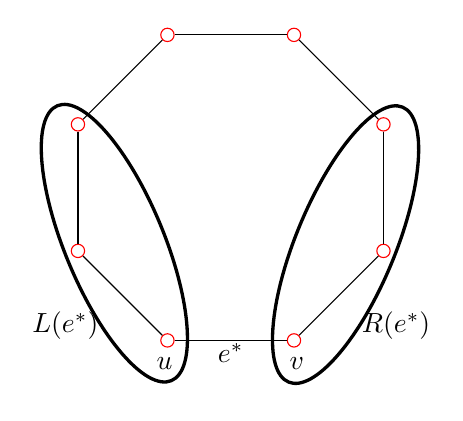
\begin{tikzpicture}[inner sep=1.7pt,scale=.7,pre/.style={<-,shorten <=2pt,>=stealth,thick}, post/.style={->,shorten >=1pt,>=stealth,thick}]

\node at (-3,-2.5) () {$L(e^*)$};
\node at (3,-2.5) () {$R(e^*)$};
\node at (0,-3) () {$e^*$};

\node at (-1.2,-3.2) () {$u$};
\node at (1.2,-3.2) () {$v$};

%\node[red] at (0,-4.2) () {$L_R$};

\tikzstyle{every node} = [draw, circle,color=red];
\foreach \i in {1,...,8}{
\path (22.5+\i*45:3) node  (a_\i) {};
}

\draw [color=black,rotate around={45*4.5:(4.3*45:1.6)},line width=1.2] (4*45:0.8) ellipse (0.9 and 2.7);
\draw [color=black,rotate around={45*7.5:(4.3*45:1.6)},line width=1.2] (4.25*45:-2.1) ellipse (0.9 and 2.7);

%\draw [color=red,rotate around={45*6:(4.3*45:1.6)},line width=1.2] (1.1*45:1.5) ellipse (0.8 and 2);

\foreach \a/\b in {1/2, 2/3, 3/4, 4/5, 5/6, 6/7, 7/8, 8/1}{
\path (a_\a) edge  (a_\b);
}

\end{tikzpicture}
\end{center}
\caption{$L$ and $R$ for an OPT edge $e^*$.}
\label{fig:opt-augmentation}
\end{figure}

%To deal with this set of cuts, we will increase the edges of the optimal cycle in the $O$-Join to ensure their $O$-Join constraint is met when they are odd. 


For an OPT edge $\es=(u,v)$, let $L(\es)$  be the largest $\eta$-near minimum cut  (w.r.t. $z$) containing $u$ and not $v$ which is crossed on both sides. Let $R(\es)$ be the largest near minimum cut containing $v$ and not $u$ which is crossed on both sides. (Note that $L(\es),R(\es)$ do not necessarily exist). For example, see \cref{fig:opt-augmentation}. 


%\begin{theorem}[Cuts Crossed on Both Sides]\label{thm:cuts-crossed-on-both-sides}
%	There is a procedure which increases OPT edges in the $O$-Join such that for any near minimum cut $S$ (i.e. with $z^*(\delta(S)) \le 2+\eta$) that is crossed on both sides, it is either the case that $\delta(S)_T$ is even or an OPT edge in $\delta(S)$ has been increased by $\eta/4$. Furthermore, the expected increase for any OPT edge due to this procedure is at most $5\eta^2$. 
%\end{theorem}




%\begin{definition}[Left and right partition]
%	For a set $S$, define a partition of $\delta(S)$ into $S^L$ and $S^R$ such that $$S^L = \{e=(u,v) \in \delta(S) \mid u \in S, v \text{ is to the left of $u$ and to the right of the root in OPT}\}$$ 
%\end{definition}


\begin{figure}[htb]
\begin{center}
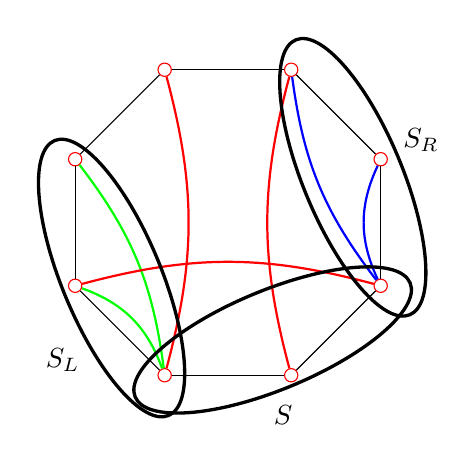
\begin{tikzpicture}[inner sep=1.7pt,scale=.7,pre/.style={<-,shorten <=2pt,>=stealth,thick}, post/.style={->,shorten >=1pt,>=stealth,thick}]

\node at (-3,-2.5) () {$S_L$};
\node at (3.5,1.5) () {$S_R$};

\node at (1,-3.5) () {$S$};

\tikzstyle{every node} = [draw, circle,color=red];
\foreach \i in {1,...,8}{
\path (22.5+\i*45:3) node  (a_\i) {};
}

\path (a_5) edge [thick, bend right=25, green] (a_4);
\path (a_5) edge [thick, bend right=15, green] (a_3);

\path (a_7) edge [thick, bend left=25, blue] (a_8);
\path (a_7) edge [thick, bend left=15, blue] (a_1);

\path (a_7) edge [thick, bend right=15, red] (a_4);
\path (a_6) edge [thick, bend left=15, red] (a_1);
\path (a_5) edge [thick, bend right=15, red] (a_2);

\draw [color=black,rotate around={45*4.5:(4.3*45:1.6)},line width=1.2] (4*45:0.8) ellipse (0.9 and 2.7);
\draw [color=black,rotate around={45*8.5:(1*45:1.6)},line width=1.2] (4.25*45:-2.1) ellipse (0.9 and 2.7);

\draw [color=black,rotate around={45*6.5:(4.3*45:1.6)},line width=1.2] (1.1*45:1.5) ellipse (0.9 and 2.7);

\foreach \a/\b in {1/2, 2/3, 3/4, 4/5, 5/6, 6/7, 7/8, 8/1}{
\path (a_\a) edge  (a_\b);
}

\end{tikzpicture}
\end{center}
\caption{$S$ is crossed on the left by $S_L$ and on the right by $S_R$. In green are edges in $\delta(S)_L$, in blue edges in $\delta(S)_R$, and in red are edges in $\delta(S)_O$. }
\label{fig:crossed-both-sides}
\end{figure}

 \begin{definition}\label{def:SLR}
 For a near minimum cut $S$ that is crossed on both sides let $S_L$ be the near minimum cut crossing $S$ on the left which minimizes the intersection with $S$, and similarly for $S_R$; if there are multiple sets crossing $S$ on the left with the same minimum intersection, choose the smallest one to be $S_L$ (and similar do for $S_R$).

% For any set $S$ crossed on both sides such that $S_L, S_R$ cross $S$ on the left and right respectively and minimize their intersections with $S$, 
We partition $\delta(S)$ into three sets $\delta(S)_L, \delta(S)_R$ and $\delta(S)_O$ as in \cref{fig:crossed-both-sides} such that
 \begin{align*}
 	\delta(S)_L &= E(S \cap S_L, S_L \smallsetminus S) \\
 	 \delta(S)_R &= E(S \cap S_R, S_R \smallsetminus S) \\
 	 \delta(S)_O &= \delta(S) \smallsetminus (\delta(S)_L \cup \delta(S)_R)
 \end{align*}

 \end{definition}
%We will increase $e$ by $\eta/4$ unless all the following hold
For an OPT edge $e^*$ define an (increase) event (of second type) $\cI_2(e^*)$ as the event that at least one of the following {\em does not} hold. (If $L(e^*)$ does not exist, assume the first and third events always hold; similarly if $R(e^*)$ does not exist, assume the second and fourth events always hold.)
\begin{equation}\label{opt-increase-event}
	%\cI_2(e^*):=\{T: 
	|T\cap \delta(L(e^*))_R| = 1, |T\cap \delta(R(e^*))_L| = 1, T\cap \delta(L(e^*))_O = \emptyset, \text{ and }T\cap \delta(R(e^*))_O = \emptyset. %\}.
\end{equation}
In the proof of \cref{thm:cutsbothsides} we will increase an OPT edge $e^*$ whenever $\cI_2(e^*)$ occurs.

\begin{lemma}\label{lem:OPT-edge-increase-prob-xed-both-sides}
For any OPT edge $e^*$, $\P{\cI_2(e^*)}\leq 18\eta$.
%Any OPT edge $e$ is increased by $\eta/4$ with probability at most $20\eta$. Therefore the expected increase of any OPT edge is at most $5\eta^2$. 	
\end{lemma}
\begin{proof}	Fix $e^*$.
To simplify notation we abbreviate $L(e^*),R(e^*)$ to $L,R$.
Since $L$ is crossed on both sides, $L_L, L_R$ are well defined. Since by \cref{lem:cutdecrement} $L_L\cap L, L_L\smallsetminus L$ are $4\eta$-near min cuts and $L$ is $2\eta$-near mincut with respect to $x$, by \cref{lem:treeoneedge}, $\P{|T\cap \delta(L)_L)|=1}\geq 1-5\eta$. Similarly, $\P{|T\cap \delta(R)_L| = 1}\geq 1-5\eta$. %Finally, 	Finally we want to condition $(\delta(L)_E)_T = 0, (\delta(R)_E)_T = 0$. By 
On the other hand, since $L, L_L, L_R$ are $2\eta$-near min cuts, by \cref{lem:nmcuts_largeedges}, $x(E(L \cap L_R, L_R)), x(E(L \cap L_L, L_L)) \ge 1-\eta$. Therefore 
$$x(\delta(L)_O) \le 2+2\eta - x(E(L \cap L_R, L_R)) - x(E(L \cap L_L, L_L)) \le 4\eta.$$ 
It follows that $\P{T\cap \delta(L)_O = \emptyset}\geq  1-4\eta$. Similarly, $\P{T\cap \delta(R)_O = \emptyset}\geq  1-4\eta$.
	Finally,	by the union bound, all events occur simultaneously with probability at least $1-18\eta$. So, $\P{\cI_2(e^*)}\leq 18\eta$ as desired.
%%	Let ${\cal A}=\{L,R,L_{R},R_{L}\}$ and ${\cal B}=\{L \cap L_{R}, R(e) \cap R_{L}, L_{R} \smallsetminus L, R_{L} \smallsetminus R\}$. Since all cuts in ${\cal A}$ are $2\eta$ near min cuts (w.r.t., $x$), by \cref{lem:cutdecrement}, all cuts in ${\cal B}$, are $4\eta$-near min cuts (w.r.t., $x$).
%	
%	Therefore, by \cref{lem:treeconditioning}, the probability that every set in ${\cal A},{\cal B}$ induces a tree simultaneously is at least $1-12\eta$. Notice that if this event occurs, it must be the case that $(\delta(L)_R)_T = 1$ and $(\delta(R)_L)_T = 1$. To see the first (the other is similar), notice when $L_R \smallsetminus L$, $L \cap L_R$ and $L_R$ are trees, the sets $L_R \smallsetminus L$ and $L \cap L_R$ share at least one edge because $L$ is connected, but at most one edge as otherwise $L$ would contain a cycle. 	
	\end{proof}


\begin{figure}[htb]\centering
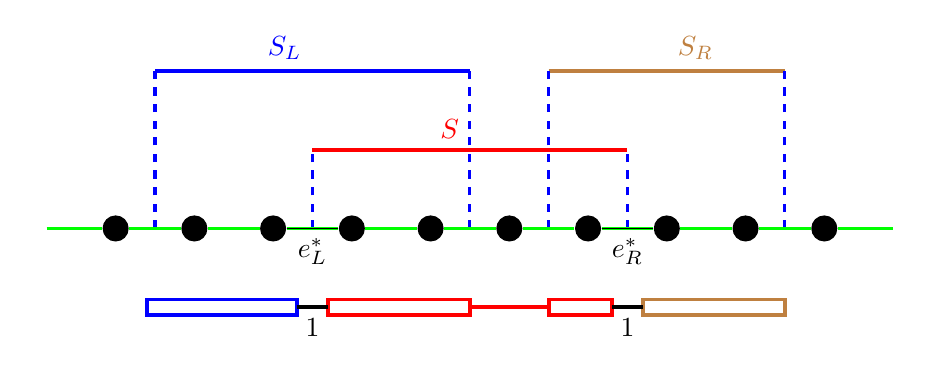
\begin{tikzpicture}
	\foreach \i in {1,...,10}{
		\node [circle,fill=black] at (\i,0) (\i) {};
	}
	\node at (0,0) (0) {}; \node at (11,0) (11) {};
	\draw [line width=1.3pt,color=red] (3.5,1) -- node [above left] {$S$} (7.5,1);
	\draw [line width=1.3pt,color=blue] (1.5,2) -- node [above left] {$S_L$} (5.5,2);
	\draw [line width=1.3pt,color=brown] (6.5,2) -- node [above right] {$S_R$} (9.5,2);
	\draw [dashed,line width=1.1pt,color=blue] (1.5,0) -- (1.5,2) (3.5,0) -- (3.5,1) (6.5,0) -- (6.5,2) (7.5,0) -- (7.5,1) (9.5,0) -- (9.5,2) (5.5,0) -- (5.5,2);
	\foreach \i/\j in {0/1,1/2,2/3,3/4,4/5,5/6,6/7,7/8,8/9,9/10,10/11}{
		\draw [color=green,line width=1.3pt] (\i) edge (\j);
		}
	\draw (3) edge node [below] {$e_L^*$} (4) (7) edge node [below] {$e_R^*$} (8);
	\draw [color=blue,line width=1.3pt] (1.4,-1.1) rectangle (3.3,-0.9);
	\draw [color=red,line width=1.3pt] (3.7,-1.1) rectangle (5.5,-0.9)
		(6.5,-1.1) rectangle (7.3,-0.9);
	\draw[color=brown,line width=1.3pt] (7.7,-1.1) rectangle (9.5,-0.9);
	\draw [line width=1.3pt] (3.3,-1)-- node [below] {$1$} (3.7,-1)
		(7.3,-1) -- node [below] {$1$} (7.7,-1);
	\draw [color=red,line width=1.3pt] (5.5,-1) -- (6.5,-1);
\end{tikzpicture}
%\begin{center}
%\begin{tikzpicture}[inner sep=1.7pt,scale=.9,pre/.style={<-,shorten <=2pt,>=stealth,thick}, post/.style={->,shorten >=1pt,>=stealth,thick}]
%\tikzstyle{every node} = [draw, circle,color=red];
%\foreach \i in {1,...,16}{
%\path (-21.5-\i*8:5) node  (a_\i) {};
%}
%
%\foreach \a in {1,...,15}{
%	\pgfmathtruncatemacro{\b}{\a + 1}
%	\path (a_\a) edge  (a_\b);
%}
%
%\foreach \a/\b/\c/\d/\e in {5.35/10.65/4.55/5.45/black, 9/12.8/4.45/5.55/red, 3/6.1/4.45/5.55/red, 5.2/14.5/4.35/5.65/blue, 1.4/10.8/4.15/5.85/orange}{
%  \draw[\e, line width=0.5mm, fill=none]
%  ($(-21.5-\a*8.5:\c cm)$) arc (-21.5-\a*8.5:-21.5-\b*8.5:\c cm)
%  --
%  ($(-21.5-\b*8.5:\d cm)$) arc (-21.5-\b*8.5:-21.5-\a*8.5:\d cm)
%  -- cycle;
%}
%
%\node[draw=none, fill=none, black] at (-89:3+1.8) () {$S$};
%\node[draw=none, fill=none, red] at (-50:3+1.7) () {$S_R$};
%\node[draw=none, fill=none, red] at (-125:3+1.6) () {$S_L$};
%
%\path (a_5) edge [color=black, ultra thick, below right] (a_6);
%\path (a_11) edge [color=black, ultra thick, below right] (a_12);
%
%\node[draw=none, fill=none, black] at (-63:3+2.3) () {$e^*_R$};
%\node[draw=none, fill=none, black] at (-116:3+2.3) () {$e^*_L$};
%
%\node[draw=none, fill=none, orange] at (-28:3+1.3) () {$R$};
%\node[draw=none, fill=none, blue] at (-150:3+1.3) () {$L$};
%
%\end{tikzpicture}
%\end{center}
\caption{Setting of \cref{lem:xed-both-sides-one-increases}. Here we zoom in on a portion of the optimal cycle and assume the root is not shown. If $\cI_2(e_L^*)$ does not occur then $E(S\cap S_L, S_L\smallsetminus S)_T=1$.}
%The lemma shows that unless $\delta(S)_T=2$, $e^*_L$ or $e^*_R$ will increase.}
\label{fig:xed-both-sides-proof}
\end{figure}


\begin{lemma}\label{lem:xed-both-sides-one-increases} Let $S$ be a cut which is crossed on both sides and let $e^*_L,e^*_R$ be the OPT edges on its interval where $e^*_L$ is the edge further clockwise. Then, if $\delta(S)_T \not=2$, at least one of $\cI_2(e^*_L),\cI_2(e^*_R)$  occurs.
\end{lemma}
\begin{proof}
%We will refer to $S_L,S_R$ as defined above. 
We prove by contradiction. Suppose none of $\cI_2(e^*_L),\cI_2(e^*_R)$ occur; we will show that this implies $\delta(S)_T = 2$. 

Let $R=R(e^*_L)$; note that $S$ is a candidate for $R(e^*_L)$, so $S\subseteq R$. Therefore, $S_L = R_L$ and we have
$$\delta(R)_L = E(R \cap R_L, R_L \smallsetminus R) = E(R \cap S_L, S_L \smallsetminus R) = \delta(S)_L.$$
where we used $S\cap S_L=R\cap S_L$ and that $S_L \smallsetminus S = S_L \smallsetminus R$.
Similarly let $L=L(e^*_R)$, and, we have $\delta(L)_R=\delta(S)_R$.

Now, since $\cI_2(e^*_L)$ has not occurred,
$1 = |T\cap \delta(R)_L| =|T\cap \delta(S)_L|,$
and since $\cI_2(e^*_R)$ has not occurred,
$1 = |T\cap \delta(L)_R|= |T\cap \delta(S)_R|,$
where  $L = L(e_R^*)$.
So, to get $\delta(S)_T=2$, it remains to show that  $T\cap \delta(S)_O = \emptyset$.
Consider any edge $e=(u,v)\in \delta(S)_O$ where  $u \in S$. We need to show $e\notin T$. Assume that $v$ is to the left of $S$ (the other case can be proven similarly). 
Then $e \in \delta(R)$. So, since $e$ goes to the left of $R$, either $e \in E(R \cap R_L, R_L \smallsetminus R)$ or $e \in \delta(R)_O$. But since $e\notin \delta(S)_L = \delta(R)_L$, we must have $e\in \delta(R)_O$. So, since $\cI_2(e^*_L)$ has not occurred, $e\notin T$ as desired.
%Then either:
%\begin{enumerate}
%\item $v$ is to the left of $S$. Then $e \in \delta(R)$, and either $e \in E(R \cap R_L, R_L \smallsetminus R)$ or $e \in \delta(R)_E$.
%\item $v$ is to the right of $S$. Then $e \in \delta(L)$, and either $e \in E(L \cap L_R, L_R \smallsetminus L)$ or $e \in \delta(L)_E$. 
%\end{enumerate}
%The first simply follows from the fact that if $v$ is to the left of $S$, it cannot be in $E(R \cap R_L, R_L \smallsetminus R)$ as $R_L$ crosses $R$ on the right side (and does not contain the root).
%
%But now this implies that any edge in $\delta(S)$ which is not a member of $E(R \cap R_L, R_L \smallsetminus R)$ or $E(L \cap L_R, L_R \smallsetminus L)$ is 0. Therefore if neither $e_L$ or $e_R$ is increased it must be that $\delta(S)_T = 2$. 
\end{proof}

\begin{proof}[Proof of \cref{thm:cutsbothsides}]
For any OPT edge $e^*$  whenever $\cI_2(e^*)$ occurs, define $s^*_{e^*}=2.02\decrease $. Then, 
by \cref{lem:OPT-edge-increase-prob-xed-both-sides}, 
$\E{s_{e^*}} \leq 18 \cdot 2.02\beta$ and for any $2\eta$-near min cut $S$ (w.r.t., $x$) that is crossed on both sides if $\delta(S)_T$ is odd, then at least one of $\cI_2(e^*_L),\cI_w(e^*_R)$ occurs, so
$$ s(\delta(S)) + s^*(\delta(S)) \geq  - x(\delta(S))\beta + s^*_{e^*_L}+s^*_{e^*_R} \geq -(2+2\eta)\decrease + 2.02\decrease \geq 0$$
for $\eta<1/100$ as desired.
%and \cref{lem:xed-both-sides-one-increases} together prove \cref{thm:cuts-crossed-on-both-sides}, which completes the goal of this section. 
\end{proof}

%Every OPT edge is an outside edge in the polygon. Look at its top two cuts $L,R$. Then consider the sides on which $L,R$ are crossed. For each such side and crossing, ensure that all partitions are trees. For each $L,R$ that is crossed, ensure that inside edges violating the parities are not picked. More formally, we will partition the edges of $\delta(L)$ into three segments: $S_L,S_R,S_i$. $S_L$ consists of all edges going into a set crossing $L$ on the left, similarly for $S_R$. We will want $S_L,S_R$ to pick exactly one edge from the ``first" crossing. If both $S_L,S_R$ are non-empty then we will want no edges from $S_i$ to be sampled, otherwise we will have no constraints on $S_i$. 


\subsection{Proof of the Main Technical Theorem, \cref{thm:maintechnical}}
The following theorem is the main result of this section.
\begin{restatable}{theorem}{beforetechnical}\label{lem:beforetechnicalthm}
Let $x^0$ be a feasible solution of the \ref{eq:tsplp} with support $E_0=E\cup\{e_0\}$ and $x$ be $x^0$ restricted to $E$.
Let $\mu$ be the max entropy distribution with marginals $x$.
For $\eta\leq 10^{-12}$, $\decrease > 0$, there is a set $E_g\subset E\smallsetminus \delta(\{u_0,v_0\})$  of {\em good} edges
%\footnote{The edge sets $E_g$ and $E^*$ need not be disjoint.} with $x_e > 0$. 
and two functions $s: E_0\rightarrow \R$ and $s^*: E^* \rightarrow \R _{\ge 0}$ (as functions of $T\sim\mu$) such that
	\begin{itemize}
\item[(i)] 	For each edge $e \in E_g$, $s_e \ge -x_e \decrease$ and for any $e\in E\smallsetminus E_g$, $s_e=0$.
\item[(ii)] For each $\eta$-near-min-cut $S$ w.r.t. $z$, if $\delta(S)_T$ is odd, then $  s(\delta(S)) + s^*(\delta(S)) \ge  0.$
\item[(iii)] We have $\E{s_e} \le -\epsilon_P \decrease x_e$  for all edges $e \in E_g$  and $\E{s^*_{e^*}} \le 218 \eta \decrease$ for all OPT edges $e^* \in E^*.$
for $\epsilon_P$ defined in \eqref{eq:epsP}.
\item[(iv)] For every $\eta$-near minimum cut $S$ of $z$ crossed on (at most) one side such that $S\neq V\smallsetminus \{u_0,v_0\}$, $x(\delta(S)\cap E_g) \ge 3/4.$
\end{itemize}
\end{restatable}
Before proving this theorem we use it to prove the main technical theorem from the previous section.
\maintechnical*
\begin{proof}[Proof of \cref{thm:maintechnical}]
Let $E_g$ be the good edges defined in \cref{lem:beforetechnicalthm} and let $E_b:=E\smallsetminus E_g$ be the set of bad edges; in particular, note all edges in $\delta(\{u_0,v_0\})$ are bad edges. We define a new vector $\tilde{s}:E\cup \{e_0\}\to\R$ as follows: 
\begin{equation}\label{eq:tildesdef}\tilde{s}(e)\gets \begin{cases}\infty & \text{if } e=e_0\\
-x_e(4\beta/5)(1-2\eta) & \text{if } e\in E_b,\\
x_e(4\beta/3) & \text{otherwise.}
\end{cases}
\end{equation}
Let $\tilde{s}^*$ be the vector $s^*$ from \cref{thm:cutsbothsides}.
We claim that for any  $\eta$-near minimum cut $S$ such that $\delta(S)_T$ is odd, we have 
$$ \tilde{s}(\delta(S))+\tilde{s}^*(\delta(S))\geq 0.$$
To check this note by (iv) of \cref{lem:beforetechnicalthm} for every set $S\neq V\smallsetminus \{u_0,v_0\}$ crossed on at most one side, we have $x(E_g \cap \delta(S)) \ge \frac{3}{4}$, so
\begin{equation}\label{eq:tildeScutsok}\tilde{s}(\delta(S))+\tilde{s}^*(\delta(S))\geq \tilde{s}(\delta(S)) = \frac{4\decrease}{3} x(E_g\cap\delta(S)) - \frac{4\decrease}{5}(1-2\eta)x(E_b\cap\delta(S))\geq 0.	
\end{equation}

For $S=V\smallsetminus \{u_0,v_0\}$, we have $\delta(S)_T=\delta(u_0)_T + \delta(v_0)_T=2$ with probability 1, so condition ii) is satisfied for these cuts as well.
Finally, consider cuts  $S$ which are crossed on both sides. By \cref{thm:cutsbothsides},
\begin{equation}\label{eq:tildeScutstwo}\tilde{s}(\delta(S)) + \tilde{s}^*(\delta(S)) \geq 0	
\end{equation}
since $\tilde{s}_e\geq -\frac{4}{5}\decrease x_e \ge -\decrease x_e$ for all $e$.

Now, we are ready to define $s,s^*$. Let $\hat{s},\hat{s}^*$ be the $s,s^*$ of \cref{lem:beforetechnicalthm} respectively.
Define $s=\gamma \tilde{s} + (1-\gamma) \hat{s}$ and similarly define $s^*=\gamma\tilde{s}^*+(1-\gamma)\hat{s}^*$ for some $\gamma$ that we choose later. 
We prove all three conclusions for $s,s^*$. (i) follows by (i) of \cref{lem:beforetechnicalthm} and  \cref{eq:tildesdef}. (ii) follows by (ii) of \cref{lem:beforetechnicalthm} and \cref{eq:tildeScutsok} above. 
%We prove all three conclusions of \cref{thm:maintechnical} for $s,s^*$. (i) follows by (i) of \cref{lem:beforetechnicalthm} and  \cref{eq:tildesdef}. (ii) follows by (ii) of \cref{lem:beforetechnicalthm} and \cref{eq:tildeScutsok,eq:tildeScutstwo} above. %\anna{This is a bit brutal. Maybe in one of the theorems switch from (i),(ii) etc to (a) (b) etc?}
It remains to verify (iii). For any OPT edge $e^*$, $\E{s^*_{e^*}}\leq 218\eta\decrease$ by (iii) of \cref{lem:beforetechnicalthm} and the construction of $\tilde{s}^*$. On the other hand, by (iii) of \cref{lem:beforetechnicalthm} and \cref{eq:tildesdef},
\begin{align*} 
\E{s_e} \begin{cases}\leq  x_e  (\gamma \frac{4}{3}\decrease - (1-\gamma)\eps_P\decrease ) & \forall e\in E_g,\\	
= -x_e\gamma\cdot (\frac{4}{5}\decrease)(1-2\eta)& \forall e\in E_b.
\end{cases}
\end{align*}
Setting $\gamma=\frac{15}{32}\eps_P$ we get $\E{s_e}\leq -\frac{1}{3}\eps_P\decrease x_e$ for $e\in E_g$ and $\E{s_e}\leq -\frac{1}{3}x_e\decrease\epsilon_P$ for $e\in E_b$ as desired.
\end{proof}
%Let $E_g$ be the good edges defined in \cref{lem:beforetechnicalthm} and let $E_b:=E\smallsetminus E_g$ be the set of bad edges. We define a new vector $\tilde{s}:E\cup \{e_0\}\to\R$ as follows: 
%\begin{equation}\label{eq:tildesdef}\tilde{s}(e)\gets \begin{cases}\infty & \text{if } e=e_0\\
%-x_e\eta/8 & \text{if } e\in E_b,\\
%x_e\eta/4 & \text{otherwise.}
%\end{cases}
%\end{equation}
%Let $\tilde{s}^*$ the vector in \cref{thm:cutsbothsides}.
%We claim that for any  $\eta$-near minimum cut $S$ w.r.t., $z$ such that $\delta(S)_T$ is odd, we have 
%$$ \tilde{s}(\delta(S))+\tilde{s}^*(\delta(S))\geq 0.$$
%To check this note by (iv) of \cref{lem:beforetechnicalthm} for every set $S\neq V\smallsetminus \{u_0,v_0\}$ crossed on at most one side, 
%\begin{equation}\label{eq:tildeScutsok}\tilde{s}(\delta(S))+\tilde{s}^*(\delta(S))\geq \tilde{s}(\delta(S)) \geq \frac{\eta}{4} \tilde{s}(E_g\cap\delta(S)) - \frac{\eta}{8}\tilde{s}(E_b\cap\delta(S))\geq 0. 	
%\end{equation}
%For $S=V\smallsetminus \{u_0,v_0\}$, we have $\delta(S)_T=\delta(u_0)_T + \delta(v_0)_T=2$ with probability 1.
%Finally, for any odd cut $S$ crossed on both sides, by \cref{thm:cutsbothsides} and the fact that $\tilde{s}_e\geq -\eta x_e/8$ for all $e$, the inequality holds. 

%Now, we are ready to define $s,s^*$. Let $\hat{s},\hat{s}^*$ be the $s,s^*$ of \cref{lem:beforetechnicalthm} respectively.
%Define $s=\alpha \tilde{s} + (1-\alpha) \hat{s}$ and similarly define $s^*=\alpha\tilde{s}^*+(1-\alpha)\hat{s}^*$ for some $\alpha$ that we choose %later. 
%We prove all three conclusions for $s,s^*$. (i) follows by (i) of \cref{lem:beforetechnicalthm} and  \cref{eq:tildesdef}. (ii) follows by (ii) %\cref{lem:beforetechnicalthm} and \cref{eq:tildeScutsok} above. 
%It remains to verify (iii). For any OPT edge $e^*$, $\E{s^*_{e^*}}\leq 45\eta^2$ by (iii) of \cref{lem:beforetechnicalthm} and the construction of $%\tilde{s}^*$. On the other hand, by (iii) of \cref{lem:beforetechnicalthm} and \cref{eq:tildesdef},
%\begin{align*} 
%\E{s_e} &\leq  x_e (\alpha\eta/4 - (1-\alpha)\eps_P\eta ), \forall e\in E_g,\\	
%\E{s_e} &= -x_e(1-\alpha)\eta/8, \forall e\in E_b.
%\end{align*}
%Setting $\alpha=\eps_P$ we get $\E{s_e}\leq -\eps_P\eta x_e/2$ for $e\in E_g$ and $\E{s_e}\leq -x_e\eta/9$ for $e\in E_b$ as desired.


\subsection{Structure of Polygons of Cuts Crossed on One Side}\label{sec:crossedOneSide}
%Since by \cref{fact:decr-below-1} the decrease in $y$ on any near minimum cut is upper bounded by $\eta/4$, this implies that we can ignore cuts that are crossed on both sides in the remaining argument, so long as we offset this increase of cost. We will employ the procedure in \cref{thm:cuts-crossed-on-both-sides} independently of all others. In other words, it does not interact with other increase and decrease procedures in this paper. 
%Following this, every cut of interest is crossed on {\em at most} one side. We now partition the remaining cuts into connected components, according to the following:
%In the rest of the section we work with near minimum cuts of $z$ crossed on one side.

\begin{definition}[Connected Component of Crossing Cuts]
	Given a family of cuts crossed on at most one side, construct a graph where two cuts are connected by an edge  if they cross. Partition this graph into {\em maximal connected components}.
	We call a path in this graph, a {\em path of crossing cuts}.
%	Let ${\cal C}$ be a family of cuts on vertices of a graph $G$.
%	For two cuts $A,B\in {\cal C}$ we say there is a path of crossing cuts from $A$ to $B$ if there is a path $A=C_0, \dots, C_k=B$ (for some $k\geq 1$) such that for any $0\leq i<k$, $C_i$ crosses $C_{i+1}$.
\end{definition}

%\begin{figure}
%\begin{center}
%\begin{tikzpicture}[inner sep=1.7pt,scale=.7,pre/.style={<-,shorten <=2pt,>=stealth,thick}, post/.style={->,shorten >=1pt,>=stealth,thick}]
%\tikzstyle{every node} = [draw, circle,color=red];
%\foreach \i in {1,...,16}{
%\path (22.5+\i*22.5:3) node  (a_\i) {};
%}
%
%\foreach \a/\b in {1/0, 3/1, 6/2, 8/3, 10/4, 12/5, 15/6}{
%\node[draw=none] at (3*22.5+\a*22.5:3+1.4) () {$a_\b$};
%}
%
%\path (22.5+3*22.5:3) node[black, fill]  (a_r) {};
%
%\foreach \i in {2,6,9, 13}{
%\draw [color=blue,rotate around={22.5*\i:(\i*22.5:2.8)},line width=1.2] (\i*22.5:2.8) ellipse (.5 and 1.7);
%}
%
%\draw [color=blue,rotate around={11.25*31:(31*11.25:2.8)},line width=1.2] (31*11.25:2.9) ellipse (.5 and 1);
%
%\draw [color=blue,rotate around={22.5*11:(22.5*11:2.9)},line width=1.2] (22.5*11:2.9) ellipse (.5 and .5);
%
%\foreach \a/\b/\c/\d/\e in {3.5/-1.5/2.25/3.5/red, 3.6/-8.5/2/3.75/red, -5.5/-11.5/2.25/3.5/black, 0.5/-11.6/1.75/4/black, 0.4/-4.5/2.15/3.65/black}{
%  \draw[\e, line width=0.5mm, fill=none]
%  ($(\a*22.5:\c cm)$) arc (\a*22.5:\b*22.5:\c cm)
%  --
%  ($(\b*22.5:\d cm)$) arc (\b*22.5:\a*22.5:\d cm)
%  -- cycle;
%}
%
%\foreach \a/\b in {1/2, 2/3, 3/4, 4/5, 5/6, 6/7, 7/8, 8/9, 9/10, 10/11, 11/12, 12/13, 13/14, 14/15, 15/16, 16/1}{
%\path (a_\a) edge  (a_\b);
%}
%
%\end{tikzpicture}\hspace*{15mm}
%\begin{tikzpicture}[inner sep=1.7pt,scale=.7,pre/.style={<-,shorten <=2pt,>=stealth,thick}, post/.style={->,shorten >=1pt,>=stealth,thick}]
%\tikzstyle{every node} = [draw, circle,color=blue, fill];
%\foreach \a\b in {1/0,2/1,3/2,4/3,5/4,6/5,7/6}{
%	\path (38+\a*51.42:3) node  (a_\a) {};
%	\node[draw=none, fill=none] at (38+\a*51.42:3+1.5) () {$a_\b$};
%}
%%, , 0.5/-11.6/1.75/4/black, 0.4/-4.5/2.15/3.65/black
%\path (38+1*51.42:3) node[black, fill]  (a_r) {};
%\foreach \a/\b/\c/\d/\e in {0.5/-1.5/2.25/3.5/red, 0.6/-4.5/2/3.75/red, -3.5/-5.5/2.25/3.5/black, -0.5/-5.6/1.75/4/black, -0.6/-2.5/2.15/3.65/black}{
%  \draw[\e, line width=0.5mm, fill=none]
%  ($(38+\a*51.42:\c cm)$) arc (38+\a*51.42:38+\b*51.42:\c cm)
%  --
%  ($(38+\b*51.42:\d cm)$) arc (38+\b*51.42:38+\a*51.42:\d cm)
%  -- cycle;
%}
%
%\foreach \a/\b in {1/2, 2/3, 3/4, 4/5, 5/6, 6/7, 7/1}{
%\path (a_\a) edge  (a_\b);
%}
%\end{tikzpicture}
%
%\end{center}
%\caption{An example of a polygon. \textit{On the left:} the red vertices represent possibly contracted sets in $\mathcal{L}$, and the blue cuts represent atoms, which are $2+14\eta=2+\eps_\eta$ near minimum cuts in $x$ by \cref{lem:smallatoms}. The black cuts represent near minimum cuts open on the left, in red near minimum cuts open on the right. The solid black circle is the root of the polygon. %, \anna{which may or may not be a vertex}. 
%\textit{On the right:} we contract the atoms for a clearer picture. By \cref{thm:poly-structure}, every edge represented in this picture is at least $1-14\eta=1-\eps_\eta$ in $x$.}
%\label{fig:polygon-example}
%\end{figure}

In the rest of this section we will focus on a single connected component ${\cal C}$ of cuts crossed on (at most) one side.
%Now let ${\cal C}$ be a connected component of near min cuts, i.e., for any two cuts $A,B\in {\cal C}$ there is a path of crossing cuts from $A$ to $B$. We define a {\em polygon} on cuts in ${\cal C}$:
\begin{definition}[Polygon]\label{def:polygon}
	For a connected component ${\cal C}$ of crossing near min cuts that are crossed on one side, let 
$a_0,\dots,a_{m-1}$  be the coarsest partition of the vertices $V$	, such that for all $0\leq i\leq m-1$ and for any $A\in {\cal C}$ either $a_i\subseteq A$ or $a_i\cap A=\emptyset$. These are called atoms. We assume $a_0$ is the atom that contains the special edge $e_0$, and we call it the {\em root}. 
	Note that for any $A\in {\cal C}, a_0\cap A=\emptyset$. 
	
	Since every cut $A\in {\cal C}$ corresponds to an interval of vertices in $V$ in the optimum Hamiltonian cycle, we can arrange $a_0,\dots,a_{m-1}$ around a cycle (in the counter clockwise order). We label the arcs in this cycle from 1 to m, where $i+1$ is the arc connecting $a_i$ and $a_{i+1}$  (and $m$ is the name of the arc connecting $a_{m-1}$ and $a_0$). Then every cut $A\in {\cal C}$ can be identified by the two arcs surrounding its atoms. %Note that we can specify a cut $(A,\overline{A})$ by each of its sides. %We choose the convention to choose the side that does not have the root. 
	 Specifically, $A$ is identified with arcs $i,j$ (where $i<j$) if $A$ contains  atoms $a_{i},\dots, a_{j-1}$, and we write  $\ell(A)=i, r(A)=j$. Note that  $A$ does not contain the root $a_0$. 
	
	By construction for every arc $1\leq i\leq m$, there exists a cut $A$ such that $\ell(A)=i$ or $r(A)=i$. Furthermore, $A,B\in {\cal C}$ (with $\ell(A)\leq \ell(B)$) cross iff $\ell(A) < \ell(B)<r(A)<r(B)$.
	
	See \cref{fig:polygon-example-detail} for a visual example.
\end{definition}

Notice that every atom of a polygon is an interval of the optimal cycle.
In this section, we prove the following structural theorem about polygons of near minimum cuts crossed on one side. 
% and then we use it to construct the $\ss$ vector. 
% Suppose not, and suppose that the leftmost vertex of an atom is $v_i$ and the rightmost $v_j$, but some vertex $v_k$ between $v_i,v_j$ is not a member of the atom. Then there is some cut along the optimal cycle which separates $v_i$ and $v_k$. Yet it must also separate $v_i$ and $v_j$, which contradicts the definition of an atom.

\begin{theorem}[Polygon Structure]\label{thm:poly-structure}
For  $\eps_{\eta}\geq 14\eta$ and any polygon with atoms $a_0...a_{m-1}$ (where $a_0$ is the root) the following holds:
	\begin{itemize}
	\item For all adjacent atoms $a_i,a_{i+1}$ (also including $a_0,a_{m-1}$), we have $x(E(a_i,a_{i+1})) \ge 1-\eps_\eta$. 
	\item All atoms $a_i$ (including the root) have $x(\delta(a_i)) \le 2+\eps_\eta$. 
	\item $x(E(a_0, \{a_2,\dots,a_{m-2}\}))\leq \eps_{\eta}$.
 %In addition $x(\{a_0...a_{m-1}\}) \le 2+\eps_\eta$. 
	\end{itemize}
\end{theorem}
The interpretation of this theorem is that the structure of a polygon converges to the structure of an actual integral cycle as $\eta\to 0$. 
The proof of the theorem follows from the lemmas in the rest of this subsection.

%Our remaining minimum cuts consist of a collection of polygons and cuts that are not crossed.  In \cref{sec:crossedOneSide} we will prove structural properties of polygons. One important property we prove is the following:




%Here we prove properties of polygons (see \cref{def:polygon}). 
%For the rest of this subsection, fix a connected component ${\cal C}$ of near min cuts of $z^*$ with $m$ atoms $a_0,\dots,a_{m-1}$ and  $m$ arcs $1,\dots, m$. See \cref{fig:polygon-example} for an example with and without atoms contracted.

\begin{figure}[htb]
	\centering
	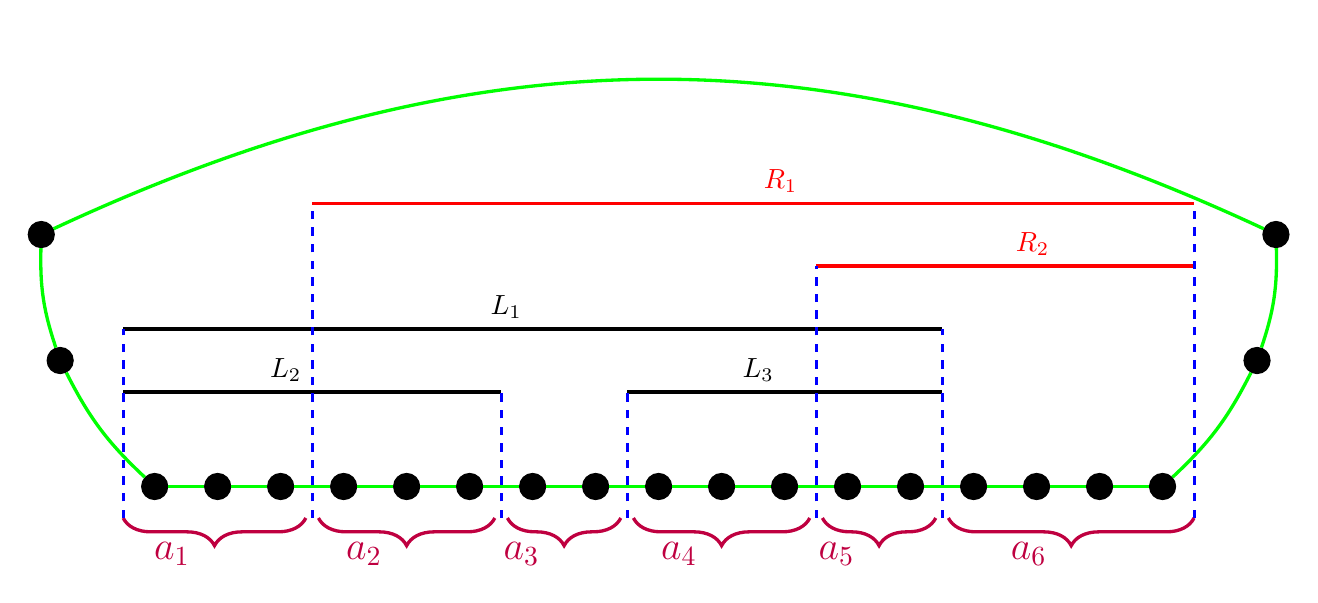
\begin{tikzpicture}[scale=0.8]
		\foreach \i in {3,...,19}{
			\node [draw,fill=black,circle] at (\i,0) (\i) {};
		}
		\node [draw,fill=black,circle] at (1.2,4) (1) {};
		\node [draw,fill=black,circle] at (1.5,2) (2) {};
		\node [draw,fill=black,circle] at (20.5,2) (20) {};
		\node [draw,fill=black,circle] at (20.8,4) (21) {};

	   \foreach \i/\j in {3/4,4/5,5/6,6/7,7/8, 8/9, 9/10, 10/11, 11/12, 12/13, 13/14, 14/15, 15/16, 16/17, 17/18, 18/19}{
	   	\draw [color=green, line width=1.2pt] (\i) edge (\j);
	   }
	   \draw [color=green, line width=1.2pt] (1) edge [bend left=25] (21)
	   (1) edge [bend right=10] (2) (2) edge [bend right=10] (3) (19) edge [bend right=10] (20) (20) edge [bend right=10] (21);
		\draw [line width=1.1pt] (2.5,2.5) -- node [above left] {$L_1$} (15.5,2.5) 
		(2.5,1.5) -- node [above left] {$L_2$} (8.5,1.5)
		(10.5,1.5) -- node [above left] {$L_3$} (15.5,1.5)
		;
		\draw[ line width=1.1pt, color=red] (5.5,4.5) -- node [above right] {$R_1$} (19.5,4.5)
		(13.5,3.5) -- node [above right] {$R_2$} (19.5,3.5);
		\foreach \i/\a/\b in {1/2.5/5.4, 2/5.6/8.4, 3/8.6/10.4, 4/10.6/13.4, 5/13.6/15.4, 6/15.6/19.5}{
			\draw [line width=1.2pt, color=purple,decorate,decoration={brace,amplitude=10pt}]
(\b,-0.5) -- node [below left=5] {\Large$a_\i$} (\a,-0.5);
}		
		\draw [dashed,color=blue,line width=1.1pt] (2.5,-0.5) -- (2.5,2.5)
		(5.5,-0.5) -- (5.5,4.5) (8.5,-0.5) -- (8.5,1.5) (10.5,-0.5) -- (10.5,1.5)  (19.5,-0.5) -- (19.5,4.5) (13.5,-0.5) -- (13.5,3.5) (15.5,-0.5) -- (15.5,2.5);
	\end{tikzpicture}\vspace{0.5cm} 
	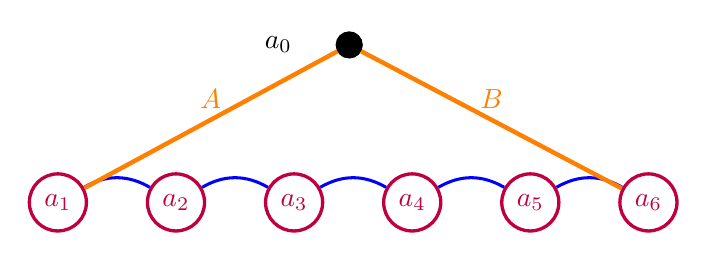
\begin{tikzpicture}
	  \node [draw,fill=black,circle] at (3.7,2) (a0) {};
	  \foreach \i/\j in {0/1, 1/2, 2/3, 3/4, 4/5, 5/6}{
	  	\node [draw,circle,color=purple,line width=1.2pt] at (1.5*\i,0) (a\j) {$a_{\j}$};
	  }
	 \foreach \i/\j in {1/2, 2/3, 3/4, 4/5, 5/6}{
	  	\draw [line width=1.1pt, color=blue] (a\i) edge [bend left=30] (a\j);
	  }
	  \node at (2.8,2) () {$a_0$};
	\draw [line width=1.6pt, color=orange] (a1) edge node [above] {$A$} (a0) (a6) edge node [above] {$B$} (a0); 
	\end{tikzpicture}
	\caption{An example of a polygon with contracted atoms. In black are the cuts in the left polygon hierarchy, in red the cuts in the right polygon hierarchy. OPT edges around the cycle are shown in green.
	Here $R_1$ is an ancestor of $R_2$, however it is not a strict ancestor of $R_2$ since they have the same right endpoint. $L_1$ is a strict ancestor and the strict parent of $L_3$. By \cref{thm:poly-structure}, every edge in the bottom picture represents a set of LP edges of total fraction at least $1-\eps_\eta$.  }
\label{fig:polygon-example-detail}
\end{figure}

%\begin{figure}[htb]
%\begin{center}
%\begin{tikzpicture}[inner sep=1.7pt,scale=.7,pre/.style={<-,shorten <=2pt,>=stealth,thick}, post/.style={->,shorten >=1pt,>=stealth,thick}]
%\tikzstyle{every node} = [draw, circle,color=blue, fill];
%\foreach \a\b in {1/0,2/1,3/2,4/3,5/4,6/5,7/6}{
%	\path (38+\a*51.42:3) node  (a_\a) {};
%	\node[draw=none, fill=none] at (38+\a*51.42:3+1.5) () {$a_\b$};
%}
%%, , 0.5/-11.6/1.75/4/black, 0.4/-4.5/2.15/3.65/black
%\path (38+1*51.42:3) node[black, fill]  (a_r) {};
%\foreach \a/\b/\c/\d/\e in {0.5/-1.5/2.25/3.5/red, 0.6/-4.5/2/3.75/red, -3.5/-5.5/2.25/3.5/black, -0.5/-5.6/1.75/4/black, -0.6/-2.5/2.15/3.65/black}{
%  \draw[\e, line width=0.5mm, fill=none]
%  ($(38+\a*51.42:\c cm)$) arc (38+\a*51.42:38+\b*51.42:\c cm)
%  --
%  ($(38+\b*51.42:\d cm)$) arc (38+\b*51.42:38+\a*51.42:\d cm)
%  -- cycle;
%}
%
%\node[draw=none, fill=none, red] at (50:3+0.2) () {$R_1$};
%\node[draw=none, fill=none, red] at (50:3+1.1) () {$R_2$};
%
%
%\node[draw=none, fill=none, black] at (-51.42*3+72:3+0.2) () {$L_1$};
%\node[draw=none, fill=none, black] at (-51.42*3+68:3+1.4) () {$L_2$};
%
%\foreach \a/\b in {1/2, 2/3, 3/4, 4/5, 5/6, 6/7, 7/1}{
%\path (a_\a) edge node[draw=none,fill=white]{\textcolor{gray}{\a}} (a_\b);
%}
%\end{tikzpicture}
%
%\end{center}
%\caption{An example of a polygon with contracted atoms. In black are the cuts in the left polygon hierarchy, in red the cuts in the right polygon hierarchy. We have labeled the arcs in gray. $R_1$ is the cut containing atoms $a_5,a_6$ and $R_2$ is the cut containing atoms $a_2...a_6$. Then $R_2$ is an ancestor of $R_1$, however it is not a strict ancestor of $R_1$ since they have the same right endpoint. $L_1$ is the cut containing atoms $a_4,a_5$ and $L_2$ is the cut containing atoms $a_1...a_5$. Then $L_2$ is a strict ancestor and the strict parent of $L_1$.}
%\label{fig:polygon-example-detail}
%\end{figure}

\begin{definition}[Left and Right  Hierarchies]
For a polygon $u$ corresponding to a connected component ${\cal C}$ of cuts crossed on one side, let ${\cal L}$ (the {\em left  hierarchy}) be the set of all  cuts $A\in {\cal C}$ that are not crossed on the left.
We call any cut in ${\cal L}$ {\em open} on the left. Similarly, we let ${\cal R}$ be the set of  cuts that are open on the right.
So, ${\cal L},{\cal R}$ is a partitioning of all cuts in ${\cal C}$. 
%such  and there does not exist a near tight set $S'$ with $r \not\in S'$ which crosses $S$ such that $S'$ contains a node closer to the root clockwise. 

For two distinct cuts $A,B\in {\cal L}$ we say $A$ is an {\em ancestor} of $B$ in the left polygon hierarchy if $A\supseteq B$. We say $A$ is a {\em strict} ancestor of $B$ if, in addition, $\ell(A) \not= \ell(B)$. We define the right  hierarchy similarly: $A$ is a strict ancestor of $B$ if $A \supseteq B$ and $r(A) \not= r(B)$. 

We say $B$ is a {\em strict parent} of $A$ if among all strict ancestors of $A$ in the (left or right) hierarchy, $B$ is the one closest to $A$.

See \cref{fig:polygon-example-detail} for examples of sets and their parent/ancestor relationships. 
\end{definition}

\begin{fact}\label{lem:same-hieararchy-no-cross}
If $A,B$ are in the same hierarchy and they are not ancestors of each other, then $A\cap B=\emptyset$.	
\end{fact}
\begin{proof}
If $A\cap B\neq \emptyset$ then they cross. So, they cannot be open on the same side.
\end{proof}
This lemma immediately implies that the cuts in each of the left (and right) hierarchies form a laminar family.

\begin{lemma}\label{lem:ABcommoncross}
For $A, B\in {\cal R}$  where $B$ is a strict parent of $A$, there exists a cut $C\in {\cal L}$ that crosses both $A,B$. Similarly, if $A,B \in {\cal L}$ and $B$ is a strict parent of $A$, there exists a cut $C \in {\cal R}$ that crosses $A,B$.
\end{lemma}
\begin{proof}
Since we have a connected component of near min cuts, there exists a path of crossing cuts from $A$ to $B$. Let $P=(A=C_0, C_1,\dots, C_k=B)$ be the shortest such path. We need to show that $k=2$. 
%First, observe that for every odd $i$, $C_i\in {\cal L}$ (and for every even $i$, $C_i\in {\cal R}$). 

First, since $C_1$ crosses $C_0$ and $C_0$ is open on right, we have
$$ \ell(C_1) < \ell(C_0) < r(C_1) < r(C_0).$$
Let $I$ be the {\em closed} interval $[\ell(C_1),r(C_0)]$. Note that $C_k=B$ has an endpoint that does not belong to $I$. Let $C_i$ be the {\em first} cut in the path with an endpoint not in $I$ (definitely $i>1$).
This means $C_{i-1}\subseteq I$; so, since $C_{i-1}$ crosses $C_i$,  exactly one of the endpoints of $C_i$ is strictly inside $I$. We consider two cases:

{\bf Case 1: $r(C_{i}) > r(C_0)$.} In this case, $C_i$ must be crossed on the left (by $C_{i-1}$) and $C_{i}\in {\cal R}$ and it does not cross $C_0$. So, $C_0\subsetneq C_i$ and
 $$\ell(C_1) < \ell(C_i)\leq \ell(C_0)$$
 where the first inequality uses that the left endpoint of $C_i$ is strictly inside $I$. Therefore, $C_1$ crosses both of $C_0,C_i$, and $C_i$ is a strict ancestor of $A=C_0$. If $C_i=B$ we are done, otherwise, $A\subseteq B \subseteq C_i$, but since $C_1$ crosses both  $A$ and $C_i$, it also crosses $B$ and we are done.

{\bf Case 2: $\ell(C_i)<\ell(C_1)$.} In this case, $C_i$ must be crossed on the right (by $C_{i-1}$) and $C_i\in {\cal L}$ and it does not cross $C_1$. So, we must have
$$ r(C_1) \leq r(C_i) < r(C_0), $$
where the second inequality uses that the right endpoint of $C_i$ is strictly inside $I$. But, this implies that $C_i$ also crosses $C_0$. So, we can obtain a shorter path by excluding all cuts $C_1,\dots, C_{i-1}$ and that is a contradiction.
%\end{description}
%We prove this for the case $A, B\in {\cal R}$ (the other case is similar). Since we have a connected family of near minimum cuts, there exists a path of crossing cuts from $A$ to $B$. Let $P=(A=C_0, C_1,\dots, C_k=B)$ be the shortest such path. We need to show that $k=2$. By way of contradiction suppose $k \ge 3$ 
%
%First, observe that $C_1,C_3 \in {\cal L}$ and $C_0,C_2 \in {\cal R}$. By \cref{lem:same-hieararchy-no-cross}, $A=C_0$ and $C_2$ may not cross. We now show $C_0 \subseteq C_2$. Since $C_2$ crosses $C_1$ on the right, $r(C_2) > r(C_1)$, and $l(C_2) < r(C_1)$. Since $r(C_1) > l(C_0)$, we must have $r(C_2) > l(C_0)$, and similarly $l(C_2) < r(C_0)$. Therefore, they are not disjoint. Now suppose $C_2 \subseteq C_0$. Since $B$ ends strictly to the right of $C_0$, there must be some cut $C_k$ in the path of cuts from $A$ to $B$ which crosses the interval $C_0 \cup C_1$. But $C_k$ must cross either $C_0$ or $C_1$, contradicting that $C_2$ is in the shortest path. It follows that $C_0 \subseteq C_2$. 
%
%This implies $r(C_0) = r(C_2)$, as otherwise this would contradict that $B$ is the strict parent of $A$.
%
%Now consider $C_3$. It must cross $C_2$ on the left. However, it cannot cross $C_1$ on the left, as $C_1 \in {\cal L}$. Therefore, $r(C_3) \ge r(C_1) > l(C_0)$. Therefore since $r(C_0)=r(C_2)$, $C_3$ must cross $C_0$ (we cannot have $C_3 \subseteq C_0$ as $l(C_3) \le l(C_2) \le l(C_0)$). This contradicts that $P$ is the shortest path, completing the proof.
%First, since $C_1$ crosses $C_0$ and $C_0$ is open on right, we have
%$$ \ell(C_1) < \ell(C_0) < r(C_1) < r(C_0).$$
%Let $I$ be the {\em closed} interval $[\ell(C_1),r(C_0)]$. Note that $C_k=B$ has an endpoint that does not belong to $I$. Let $C_i$ be the {\em first} cut with an endpoint not in $I$ (definitely $i>1$).
%This means $C_{i-1}\subseteq I$; so, since $C_{i-1}$ crosses $C_i$,  exactly one of the endpoints of $C_i$ is strictly inside $I$. We consider two cases:
%\begin{description}
%\item [Case 1: $r(C_{i}) > r(C_0)$.] In this case, $C_i$ must be crossed on the left (by $C_{i-1}$) and $C_{i}\in {\cal R}$ and it does not cross $C_0$. So, $C_0\subsetneq C_i$ and
% $$\ell(C_1) < \ell(C_i)\leq \ell(C_0)$$
% where the first inequality uses that the left endpoint of $C_i$ is strictly inside $I$. Therefore, $C_1$ crosses both of $C_0,C_i$, and $C_i$ is a strict ancestor of $A=C_0$. If $C_i=B$ we are done, otherwise, $A\subseteq B \subseteq C_i$, but since $C_1$ crosses both of $A,C_i$, it also crosses $B$ and we are done.
% \item [Case 2: $\ell(C_i)<\ell(C_1)$.] In this case, $C_i$ must be crossed on the right (by $C_{i-1}$) and $C_i\in {\cal L}$ and it does not cross $C_1$. So, we must have
%$$ r(C_1) \leq r(C_i) < r(C_0), $$
%where the second inequality uses that the right endpoint of $C_i$ is strictly inside $I$. But, this implies that $C_i$ also crosses $C_0$. So, we can obtain a shorter path by excluding all cuts $C_1,\dots, C_{i-1}$ and that is a contradiction.
%\end{description}
\end{proof}

\begin{lemma}\label{lem:ABcommonancestor}
Let $A,B\in {\cal R}$ such that $A\cap B=\emptyset$, i.e., they are not ancestors of each other. Then, they have a common ancestor, i.e., there exists a set $C\in {\cal R}$ such that $A,B\subseteq C$.	
\end{lemma}
\begin{proof}
WLOG assume $r(A)\leq \ell(B)$.
Let $C$ be the highest ancestor of $A$ in the hierarchy, i.e., $C$ has no ancestor. For the sake of contradiction suppose $B\cap C=\emptyset$ (otherwise, $C$ is an ancestor of $B$ and we are done). So, $r(C)\leq \ell(B)$. Consider the path of crossing cuts from $C$ to $B$, say $C=C_0,\dots,C_k=B$. 

Let $C_i$ be the first cut in this path such that $r(C_i)>r(C_0)$. Note that such a cut always exists as $r(B)>r(C)$. 
%Since $C_{i-1}$ crosses $C_i$ and $r(C_{i-1})\leq r(C_0)$, we must have $C_i\in {\cal R}$. Therefore, we must have $\ell(C_i)<r(C_0)$.
Since $C_{i-1}$ crosses $C_i$ and $r(C_{i-1})\leq r(C_0)$, $C_{i-1}$ crosses $C_i$ on the left and $C_i$ is open on the  right. We show that $C_i$ is an ancestor of $C=C_0$ and we get a contradiction to $C_0$ having no ancestors (in ${\cal R}$).
If $\ell(C_0)<\ell(C_i)$, then $C_i$ crosses $C_0$ on the right and that is a contradiction. So, we must have $C_0\subseteq C_i$, i.e., $C_i$ is an ancestor of $C_0$.
\end{proof}
It follows from the above lemma that each of the left and right hierarchies have a unique cut  with no ancestors.

\begin{lemma}\label{lem:strictparentexists}
If $A$ is a cut in ${\cal R}$ such that $r(A)<m$, then $A$ has a strict ancestor. And, similarly, if $A\in{\cal L}$ satisfies $\ell(A)>1$, then it has a strict ancestor.
\end{lemma}
\begin{proof}
Fix a cut $A\in {\cal R}$. If there is a cut in $B\in {\cal R}$ such that $r(B)>r(A)$, then either $B$ is a strict ancestor of $A$ in which case we are done, or $A\cap B=\emptyset$, but then by \cref{lem:ABcommonancestor} $A,B$ have a common ancestor $C$, and $C$ must be a strict ancestor of $A$ and we are done.

Now, suppose for any $R\in {\cal R}$, $r(R)\leq r(A)$. So, there must be a cut $B\in {\cal L}$ such that $r(B)>r(A)$ (otherwise we should have less than $m$ atoms in our polygon). The cut $B$ must be crossed on the right by a cut $C\in {\cal R}$. But then, we must have $r(C)>r(B)>r(A)$ which is a contradiction. 
\end{proof}


\begin{corollary}\label{cor:leftmostrightmostancestor}
	If $A\in {\cal C}$ has no strict ancestor, then $r(A)=m$ if $A\in {\cal R}$ and $\ell(A)=1$ otherwise.
\end{corollary}


%Here we prove the two lemmas from this subsection mentioned in the summary:
\begin{restatable}[Polygons are Near Minimum Cuts]{lemma}{lemNMC}\label{lem:NMC}
$x(\delta(a_1\cup\dots\cup a_{m-1}))\leq 2+4\eta.$ 
\end{restatable}
\begin{proof}
	Let $A\in {\cal L}$ and $B\in {\cal R}$ be the unique cuts in the left/right  hierarchy with no ancestors. Note that $A$ and $B$ are crossing (because there is a cut $C$ that crosses $A$ on the right, and $B$ is an ancestor of $C$). Therefore, since $A,B$ are both $2\eta$ near min cuts (with respect to $x$), by \cref{lem:cutdecrement}, $A\cup B$ is a $4\eta$ near min cut.
\end{proof} 


\begin{restatable}[Root Neighbors]{lemma}{lemrootededges}\label{lem:rootedgesarebig}
$x(E(a_0, a_1)), x(E(a_0, a_{m-1})) \geq 1-2\eta$.	
\end{restatable}
\begin{proof}
Here we prove $x(E(a_0,a_1))\geq 1-2\eta$. One can prove $x(E(a_0, a_{m-1})) \ge 1-2\eta$   similarly. Let $A\in {\cal L}$ and $B\in {\cal R}$ be the unique cuts in the left/right hierarchy with no ancestors.
First, observe that if $\ell(B)=2$, then since $A,B$ are crossing, by \cref{lem:nmcuts_largeedges} we have
$$x(E(A\smallsetminus B, \overline{A\cup B})) = x(E(a_1, a_0)) \geq 1-\eta.$$
as desired.

By definition of atoms, there exists a cut $C\in{\cal C}$ such that either $\ell(C)=2$ or $r(C)=2$; but if $r(C)=2$ we must have $\ell(C)=1$ in which case $C$ cannot be crossed, so this does not happen. So, we must have  $\ell(C)=2$. 	
If $C\in {\cal R}$, then since $C$ is a descendent of $B$, we must have $\ell(B)=2$, and we are done by the previous paragraph.

Otherwise, suppose $C\in {\cal L}$. 
%If $\ell(B)=2$ we are done as before. Otherwise, 
We claim that $B$ crosses $C$. This is because, $C$ is crossed on the right by some cut $B'$ and $B$ is an ancestor of $B'$, so $B\cap C\neq \emptyset$ and $C\not\subseteq B$ since $\ell(B)>2$. 
Therefore, by \cref{lem:cutdecrement} $B\cup C$ is a $4\eta$ near min cut. Since $A$ crosses $B\cup C$, by \cref{lem:nmcuts_largeedges} we have
$$x(E(A\smallsetminus (B\cup C), \overline{A\cup B\cup C})) = x(E(a_1, a_0)) \geq 1-2\eta$$ 
as desired.
%Let $A'$ be a strict parent of $C$ (note that we may have $A'=A$). Observe that $\ell(A')=1$. By \cref{lem:} there is a cut $D$ which crosses 
\end{proof}


\begin{lemma}\label{lem:polygonedgesarebig}
For any pair of atoms $a_i,a_{i+1}$ where $1\leq i\leq m-2$ we have $x(\delta(\{a_i,a_{i+1}\}))\leq 2+12\eta$, so $x(E(a_i,a_{i+1}))\geq 1-6\eta$.	
\end{lemma}
\begin{proof}
We prove the following claim: There exists $j\leq i$ such that $x(\delta(\{a_j,\dots,a_{i+1}\}))\leq 2+6\eta$. 
Then, by a similar argument we can find $j'\geq i+1$ such that $x(\delta(\{a_i,\dots,a_{j'}\}))\leq 2+6\eta$. By \cref{lem:cutdecrement} it follows that $x(\delta(\{a_i,a_{i+1}\}))\leq 2+12\eta$. Since $x(\delta(a_i)),x(\delta(a_{i+1}))\geq 2$, we have
$$x(\delta(\{a_i,a_{i+1}\})) + 2x(E(a_i,a_{i+1})) \ge 4.$$
But due to the bound on $x(\delta(\{a_i,a_{i+1}\}))$ we must have $x(E(a_i,a_{i+1}))\geq 1-6\eta$ as desired.


It remains to prove the claim. 	
First, observe that there is a cut $A$ separating $a_{i+1},a_{i+2}$ (Note that if $i+1=m-1$ then  $a_{i+2}=a_0$); so, either $\ell(A)=i+2$ or $r(A)=i+2$. If $r(A)=i+2$ then, $A$ is the cut we are looking for and we are done. So, assume $\ell(A)=i+2$. 

{\bf Case 1: $A\in {\cal L}.$}
Let $L\in {\cal L}$ be the strict parent of $A$. If $\ell(L)\leq i$ then we are done (since there is a cut $R\in\cR$ crossing $A,L$ on the right so $L\smallsetminus (A\cup R)$ is the cut that we want. If $\ell(L)=i+1$, then let $L'$ be the strict parent of $L$).
Then, there is a cut $R\in\cR$ crossing $A,L$ and a cut 
$R'$ crossing $L,L'$. 
%\anna{Could say from here: Since $R' \cap L, R \cap L \ne \emptyset$, $R' \cap R \ne \emptyset$, so $R'$ is an ancestor of $R$ and therefore also crosses $A$. $L'\smallsetminus (A\cup R')$ gives the desired interval and has $x(\delta(L'\smallsetminus (A\cup R'))) \le 2+6\eta$ by \cref{lem:cutdecrement}.  }
%Then, $x(\delta(A\cup R))\leq 2+4\eta$. 
%If $A\cup R$ crosses $L'$ on the right then $L'\smallsetminus (A\cup R)$ gives the desired interval and has $x(\delta(L'\smallsetminus (A\cup R))) \le 2+6\eta$ by \cref{lem:cutdecrement}. 
%Otherwise, $A\cup R\subset L'$. But then, the cut $R'$ must cross $A\cup R$ and $L'$ on the right. So, $x(A\cup R\cup R')\leq 2+6\eta$. Since this cut crosses $L'$ on the right, $L'\smallsetminus (A\cup R\cup R')$ gives us our interval, and $x(\delta(L'\smallsetminus (A\cup R\cup R'))) \le 2+8\eta$.
%Otherwise, $A\cup R\subset L'$. 
First, since both $R,R'$ cross $L$ (on the right) they have a non-empty intersection, so one of them say $R'$ is an ancestor of the other ($R$) and therefore $R'$ must intersect $A$.
On the other hand, since $R'$ crosses $L$ and $\ell(L)=i+1$, $\ell(R')\geq i+2=\ell(A)$. Since $R'$ intersect $A$, either they cross, or $A\subseteq R'$, so we must have $x(\delta(A\cup R))\leq 2+4\eta$.
Finally, since $R'$ crosses $L'$ (on the right) we have $x(\delta (L' \smallsetminus (A \cup R))) \le 2 + 6 \eta$ and $L'\smallsetminus (A\cup R)$ is our desired set.




{\bf Case 2: $A\in {\cal R}.$}
We know that $A$ is crossed on the left by, say,  $L\in {\cal L}$. 
If $\ell(L) \le i$, we are done, since then $L\smallsetminus A$ is the cut that we seek and we get $x(\delta(L\smallsetminus A))\leq 2+4\eta$.

Suppose then that $\ell(L) = i+1$. Let $L'$ be the strict parent of $L$, which must have $\ell(L') \le i$. 
If $L'$ crosses $A$, then $L' \smallsetminus A$ is the cut we seek and we get $x(\delta(L\smallsetminus A))\leq 2+4\eta$.

Finally, if $L'$ doesn't cross $A$, i.e., $r(A) \le r(L')$,
then consider the cut $R \in \cR$ that crosses $L$ and $L'$ on the right. Since $r(L) < r(A)$, and $A$ is not crossed on the right, it must be that $\ell(R) = i+2$.
In this case, $L' \smallsetminus R$ is the cut we want, and we get
$x(\delta(L'\smallsetminus R))\leq 2+4\eta$.
\end{proof}

\begin{restatable}[Atoms are Near Minimum Cuts]{lemma}{lematomsNMC}\label{lem:smallatoms}
For any $1\leq i\leq m-1$, we have $x(\delta(a_i))\leq 2+14\eta.$ 
\end{restatable}
\begin{proof}
By \cref{lem:polygonedgesarebig}, $x(\delta(\{a_i,a_{i+1}\}))\leq 2+12\eta$ (note that in the special case $i=m-1$ we take the pair $a_{i-1},a_i$). There must be a $2\eta$-near minimum cut $C$ (w.r.t., $x$) separating $a_{i}$ from $a_{i+1}$. Then either $a_i=C\cap \{a_i,a_{i+1}\}$ or $a_i=\{a_i,a_{i+1}\}\smallsetminus C$. In either case, we get $x(\delta(a_i))\leq 2+14\eta$ by \cref{lem:cutdecrement}.
\end{proof}



\def\cH{\mathcal{H}}

\subsection{Happy Polygons}
\label{sec:happypolygons}
\begin{definition}[$A,B,C$-Polygon Partition]\label{def:abcpolygonpartitioning}
Let $u$ be a polygon with atoms $a_0,\dots,a_{m-1}$ with root  $a_0$ where $a_1,a_{m-1}$ are the atoms left and right of the root.
The $A,B,C$-polygon partition of $u$ is a partition of edges of $\delta(u)$ into sets $A=E(a_1,a_0)$ and $B=E(a_{m-1},a_0)$, $C=\delta(u)\smallsetminus A\smallsetminus B$. 
%Note that by \cref{lem:rootedgesarebig}, $x(A),x(B)\geq 1-2\eta$ and combining this with \cref{lem:NMC}, $x(C) \le 8\eta$.
%We reduce $e$ by $\beta x_e$ when the following event happens: First, we condition on the polygon of $u$ inducing a tree. Then, we condition on $C=0$. Then,  we see if the max-flow event for $\alpha=\eps_M$ in \cref{lem:maxflow} is satisfied.
\end{definition}
Note that by \cref{thm:poly-structure}, $x(A),x(B)\geq 1-\eps_\eta$ and $x(C)\leq \eps_\eta$ where we set 
\begin{align}\label{def:eps-eta}
	\eps_\eta= 14\eta
\end{align}
as needed for \cref{thm:poly-structure}.
\begin{definition}[Leftmost and Rightmost cuts]
	Let $u$ be a polygon with atoms $a_0,\dots,a_{m-1}$ and arcs labelled $1,\dots,m$ corresponding to a connected component ${\cal C}$ of $\eta$-near minimum cuts (w.r.t., $z$).  We call any cut $C\in {\cal C}$ with $\ell(C)=1$ a {\em leftmost} cut of $u$ and any cut $C\in {\cal C}$ with $r(C)=m$ a {\em rightmost} cut of $u$. 
		We also call $a_1$ the leftmost atom of $u$ (resp.  $a_{m-1}$ the rightmost atom).
	%if $z(\delta(a_{1}))\leq 2+\eta$ (resp. $z(\delta(a_{m-1}))\leq 2+\eta$).
\end{definition}
Observe that by \cref{cor:leftmostrightmostancestor}, any cut that is not a leftmost or a rightmost cut has a strict ancestor. 

\begin{definition}[Happy Polygon]
Let $u$ be a polygon with polygon partition $A,B,C$.
For a spanning tree $T$, we say that $u$ is {\em happy} if 
$$A_T \text{ and } B_T \text{ odd}, C_T=0.$$

%Let $u$ be a polygon with polygon partition $A,B,C$.
We say that $u$ is {\em left-happy} (respectively {\em right-happy}) if 
$$A_T \text{ odd}, C_T=0,$$
(respectively $B_T \text{ odd}, C_T=0$).
\end{definition}

%Given these, we can state the main result of \cref{sec:crossedOneSide}:
\begin{definition}[Relevant Cuts]
Given a polygon $u$ corresponding to a connected component ${\cal C}$ of cuts crossed on one side with atoms $a_0,\dots,a_{m-1}$, define a family of relevant cuts
$${\cal C}'={\cal C}\cup \{a_i:  1\leq i\leq m-1, z(\delta(a_i))\leq 2+\eta\}.$$
\end{definition}
Note that atoms of $u$ are always $\eps_\eta/2$-near minimum cuts w.r.t., $z$ but not necessarily $\eta$-near minimum cuts.
The following theorem is the main result of this section.
\begin{restatable}[Happy Polygons and Cuts Crossed on One Side]{theorem}{thmcrossedoneside}\label{thm:crossed-one-side}
	Let $G=(V,E,x)$ for $x$ be an LP solution and  $z=(x+OPT)/2$.
	For a connected component ${\cal C}$ of near minimum cuts of $z$, let $u$ be the polygon with atoms $a_0,a_1...a_{m-1}$ with polygon partition $A,B,C$. 
	For $\mu$ an arbitrary distribution of spanning trees with marginals $x$, $\decrease > 0$, there is a random vector $s^*:E^*\to\R_{\geq 0}$ (as a function of $T\sim\mu$) such that for any vector $s:E\to\R$ where $s_e\geq -\decrease x_e$  for all $e\in E$ the following holds:
	
	% Then there is a procedure that increases OPT edges in the $O$-Join such that the following holds:
	\begin{itemize}
		\item If $u$ is happy then, for any cut $S\in {\cal C}'$ if  $\delta(S)_T$ is odd then we have $s(\delta(S))+s^*(\delta(S))\geq 0$,
		\item For any $S\in {\cal C}'$ that is not a rightmost/leftmost cut or rightmost/leftmost atom, if $\delta(S)_T$ is odd, then we have 
		$s(\delta(S))+s^*(\delta(S))\geq 0$. 
		\item For all OPT edges $e^*_2,\dots,e^*_{m-1}$ with respect to the above polygon, $\E{s^*_{e^*_i}}\leq 181\eta \decrease$. $\E{s^*_{e^*}} = 0$ for all other OPT edges.
	\end{itemize}
%	Moreover, the increase of any OPT edge due to this procedure is at most $210\eta(\eta/4)$ in expectation. 
\end{restatable} 


Before proving the above theorem, we study a special case.
\begin{lemma}[Triangles as Degenerate Polygons]\label{lem:trianglereduction}
	Let $S=X\cup Y$ where $X,Y,S$ are $\eps_{\eta}$-near min cuts (w.r.t., $x$) and each of these sets is a contiguous interval around the OPT cycle. Then, viewing $X$ as $a_1$ and $Y$ as $a_2$ (and $a_0=\overline{X\cup Y}$) the above theorem holds viewing $S$ as a degenerate polygon. %there is a random vector $s^*:E^*\to\R_{\geq 0}$ such that 
\end{lemma}
\begin{proof}
In this case $A=E(a_1,a_0), B=E(a_2,a_0), C=\emptyset$.
For the OPT edge $e^*$ between $X,Y$ we define $\cI_1(e^*)$ to be the event that at least one of $T\cap E(X)$, $T\cap E(Y)$, $T\cap E(S)$ is not a tree.
Whenever this happens we define $s^*_{e^*}=2.05 \cdot \decrease$.
If $S$ is left-happy we need to show when $\delta(X)_T$ is odd, then $s(\delta(X))+s^*(\delta(X))\geq 0$. This is because when $S$ is left-happy we have $A_T$ is odd (and $C_T=0$), so either $\cI_1(e^*)$ does not happen and $\delta(X)_T$ is even, or it happens in which case $s(\delta(X))+s^*(\delta(X))\geq 0$ as $s(\delta(X))\ge -(2+2\eta)\decrease$ and $s^*_{e^*}=2.05\decrease$.
Finally, observe that by \cref{lem:treeoneedge}, 
$\P{ {\cI_1(e^*)}}\le 3 \eps_\eta$, so
$\E{s^*_{e^*}}=3\eps_\eta \cdot 2.05\decrease \leq 87\eta \decrease$ using $\eta < 1/100$ and $\eps_\eta$ as defined in \cref{def:eps-eta}.
\end{proof}

%\anna{Need to add up the contributions from $\cI_1$ and $\cI_2$, and set to 0 otherwise.}


%Now, as in the previous section, we will increase $OPT$ edges to deal with these cuts. However, it will only be possible to immediately deal with cuts that do not include the arcs $1$ and $m$. 

%Throughout this subsection we assume $u$ is a polygon corresponding to a connected component ${\cal C}$ of $\eta$-near min cuts (w.r.t., $z$) crossed on one side with atoms $a_0,\dots,a_{m-1}$ where $a_0$ is the root.

\begin{lemma}\label{lem:Astrictpeven}
For every cut $A\in {\cal C}$ that is not a leftmost or a rightmost cut, $\P{\delta(A)_T=2} \geq 1-22\eta$.
\end{lemma}
\begin{proof}
Assume $A\in \cR$; the other case can be proven similarly. 
Let $B$ be the strict parent of $A$. By \cref{lem:ABcommoncross} there is a cut $C\in{\cal L}$ which crosses $A,B$ on their left. It follows by \cref{lem:cutdecrement} that $C \smallsetminus A, C\cap A$ are $4\eta$ near minimum cuts (w.r.t., $x$). So, by \cref{lem:treeoneedge}, $\P{E(A\cap C, C\smallsetminus A)_T=1}\geq 1-5\eta$. 
On the other hand, $B\smallsetminus (A\cup C)$ is a $6\eta$ near minimum cut and $A\smallsetminus C, B\smallsetminus C$ are $4\eta$ near min cuts (w.r.t., $x$). So, by \cref{lem:treeoneedge} $\P{E(A\smallsetminus C, B\smallsetminus (A\cup C))_T=1}\geq 1-7\eta$.

Finally,  by  \cref{lem:nmcuts_largeedges}, $x(E(A\cap C, C\smallsetminus A)), x(E(A\smallsetminus C, B\smallsetminus (A\cup C))) \geq 1-3\eta$. Since $A$ is a $2\eta$ near min cut (w.r.t., $x$), all remaining edges have fractional value at most $8\eta$, so with probability $1-8\eta$, $T$ does not choose any of them. Taking a union bound over all of these events, $\P{\delta(A)_T=2}\geq 1-22\eta$.
\end{proof}

\begin{lemma}\label{lem:atoms-even-whp}
	For any atom $a_i\in {\cal C}'$ that is not the leftmost or the rightmost atom we have
	$$\P{\delta(a_i)_T = 2} \ge 1-42\eta.$$
\end{lemma}
\begin{proof}
	%Consider the two neighbors of $a_i$, $a_{i-1}$ and $a_{i+1}$. 
	By \cref{lem:polygonedgesarebig}, $x(\delta(\{a_i,a_{i+1}\}))\leq 2+12\eta$, 
	%x(\delta(\{a_{i-1},a_i\}))  \le 2+12\eta.$$
	and by \cref{lem:smallatoms}, $x(\delta(a_{i+1}))\leq 2+14\eta$ (also recall by the assumption of lemma $x(\delta(a_i))\leq 2+2\eta$,
	 Therefore, by \cref{lem:treeoneedge}, 
	 $$\P{E(a_{i},a_{i+1})_T=1},\P{E(a_{i-1},a_i)_T=1}\geq 1-14\eta,$$
	 where the second inequality holds similarly.
%	 Similarly, $\geq 1-14\eta$.
Also, by \cref{lem:polygonedgesarebig}, $x(E(a_{i-1},a_{i})),x(E(a_{i},a_{i+1}))	 \geq 1-6\eta$.
Since $x(\delta(a_i))\leq 2+2\eta$, $x(E(a_i, \overline{a_{i-1}\cup a_i\cup a_{i+1}}))\leq 14\eta$.
So, 
$$\P{T\cap E(a_i, \overline{a_{i-1}\cup a_i\cup a_{i+1}})=\emptyset}\geq 1-14\eta.$$
%	\begin{equation}\label{loc-eq:bigedges}
%		x(E(a_i,a_{i+1})),x(E(a_{i-1},a_{i})) \ge 1-6\eta
%	\end{equation}
%	Similarly by \cref{lem:smallatoms} we know $\delta(a_{i-1}),\delta(a_{i+1}) \le 2+14\eta$. 
%Therefore, we can condition $a_{i-1},a_i,a_{i+1},\{a_{i-1},a_i\},\{a_i,a_{i+1}\}$ to be trees and $x(E(a_i,\bar{a_i}))_T = 0$ simultaneously, 
Finally,  by the union bound all events occur with probability at least $1-42\eta$. 
\end{proof}

Let $e^*_1,\dots,e^*_m$ be the OPT edges mapped to the arcs $1,\dots,m$ of the component $\cal C$ respectively.
\begin{lemma}\label{lem:4cutmapping}
There is a {\em mapping}\footnote{Each cut will be mapped to one or two OPT edges.} of cuts in ${\cal C}'$  to OPT edges $e^*_2,\dots e^*_{m-1}$ such that each OPT edge has at most 4 cuts mapped to it, an OPT edge $e^*$ is mapped to a cut $S$ only if $e^* \in \delta(S)$, and every atom of the polygon in ${\cal C}'$ gets mapped to two (not necessarily distinct) OPT edges. %\footnote{These will be one or both of the OPT edges adjacent to the atom.}
\end{lemma}
\begin{proof}
Consider first the set of cuts in $ {\cal C}'_\cR:= \cR \cup \{a_i:  1\leq i\leq m-1, z(\delta(a_i))\leq 2+\eta\}$ and similarly $ {\cal C}'_\cL:= \cL \cup \{a_i:  1\leq i\leq m-1, z(\delta(a_i))\leq 2+\eta\}$.  Observe that this is also a laminar family. Note that atoms are in both $\cC'_\cR$ and $\cC'_\cL$.
%Note that cuts assigned to $u$ are cuts in ${\cal C}=\cL\cup\cR$ together with atoms of $u$ which are near min cuts.
%For the sake of this proof we abuse notation and include all atoms of $u$ that are near min cuts to ${\cal R}$. 
%In the proof we only use that $\cR$ is a laminar family of cuts; note that this property remains valid after adding the atoms.
We  define a map from cuts in ${\cal C}'_R$  to OPT edges such that every OPT edge $e^*_2,\dots,e^*_{m-1}$ gets at most $2$ cuts mapped to it. A similar argument works for cuts in $\cC'_\cL$. %For ease of exposition, we allow cuts to be assigned to more than one edge. 

For any  $2\leq i\leq m-1$, we map 
$$\argmax_{A\in \cC'_\cR: \ell(A)=i} |A|\text{ and }\argmax_{A\in \cC'_\cR: r(A)=i} |A|$$ 
to $e^*_i$, where recall $\ell(A)$ is the OPT edge leaving $A$ on the left side and $r(A)$ the OPT edge leaving on the right. 
%(notice that no cut in ${\cal R}$ contains arc 1). 
By construction, each OPT edge gets at most two cuts mapped to it. 

Furthermore, we claim every cut $A\in {\cal C}'_\cR$ gets mapped to at least one OPT edge.
%for every cut $A \in {\cal C}$ containing arcs $i < j$ where $j \not= m$, we claim that either $A$ is the largest cut in ${\cal R}$ on the right side of $i$ or the largest cut on the left side of $j$. Suppose not: 
For the sake of contradiction let $A\in {\cal C}'_\cR$ be a cut that is not mapped to any OPT edge. First note that $a_1$ is mapped to edge $e_2^*$ (in both hierarchies) and $a_{m-1}$ is mapped to edge $e_{m-1}^*$. Otherwise, if $A\in \cR$, $\ell(A)\neq 1$. Furthermore, if $A \in \cR$ and $r(A)=m$, then $A$ is definitely the largest cut with left endpoint $\ell(A)$.
So assume, $1<\ell(A) < r(A)<m$.
Let $B=\argmax_{B\in \cC'_\cR: \ell(B)=\ell(A)} |B|$ and let $C=\argmax_{B\in \cC'_\cR: r(C)=r(A)} |C|$. Since $A$ is not mapped to any OPT edge but $B,C$ are mapped by above definition, we must have $B,C\neq A$. But that implies $A\subsetneq B,C$. And this means $B,C$ cross; but this is a contradiction with $\cR$ being a laminar family.
\end{proof}
 %If $A$ is mapped to two OPT edges in the above construction, we choose one of them arbitrarily.
 

%Finally, we assign every atom $a_i$ with $x(\delta(a_i)) \le 2+2\eta$ of the polygon to an adjacent arc in the set $2...m-1$. In this way, each arc receives two atoms in the worst case. 

\begin{definition}[Happy Cut]We say a leftmost cut $L\in \cL$  is {\em happy} if
%$$ |T\cap E(L_R\cap L, L_R\smallsetminus L)|=1, |T \cap E(L,\overline{a_0 \cup L \cup L_R})| = 0,  |T \cap E(L \smallsetminus L_R,L_R \smallsetminus L)| = 0,$$
$$E(L,\overline{a_0 \cup L})_T = 1$$
%Also,  we say the leftmost atom $a_1$ is {\em happy} if
%$$ E(a_1,a_2)_T=1, E(a_1,a_3\cup \dots\cup a_{m-1})_T=0$$
Similarly, the leftmost atom $a_1$ is {\em happy} if $E(a_1,\overline{a_0\cup a_1})_T=1$. Define  rightmost cuts in $u$ or the rightmost atom in $u$ to be happy, similarly.
\end{definition}
Note that, by definition, if leftmost cut $L$ is happy and $u$ is left happy then $L$ is even, i.e., $\delta(L)_T=2$. Similarly, $a_1$ is even if it is happy and $u$ is left-happy.

\begin{lemma}\label{lem:even-cuts-cond-on-happy}
%If $u$ is left-happy, then 
For every leftmost or rightmost cut $A$  in $u$ that is an $\eta$-near min cut w.r.t. $z$, $\P{A\text{ happy}}\geq 1-10\eta$, and for the leftmost atom $a_1$ (resp. rightmost atom $a_{m-1}$), if it is an $\eta$-near min cut then  $\P{a_1\text{ happy}}\geq 1-24\eta$ (resp. $\P{a_{m-1}\text{ happy}}\geq 1-24\eta$).
%, and similarly for right-happy and cuts without strict parents in the right polygon hierarchy. 
%The atoms $a_1,a_{m-1}$ are even with probability at least $1-24\eta$ conditioned on the left-happy and right-happy events respectively and provided $\delta(a_1) \le 2+2\eta$ (respectively, $\delta(a_{m-1}) \le 2+2\eta$). 
\end{lemma}
\begin{proof}
Recall that if $A$ is a $\eta$-near min cut w.r.t. $z$ then it is a $2\eta$-near min cut w.r.t. $x$.
Also, recall for a cut $L\in\cL$, $L_R$ is the near minimum cut crossing $L$ on the right that minimizes the intersection (see \cref{def:SLR}).
	We prove this for the leftmost cuts and the leftmost atom; the other case can be proven similarly. Consider a cut $L \in {\cal L}$. %Since $u$ is left-happy, for $A,B,C$ polygon partition of $u$, we know $A_T=(E(a_1,a_0))_T = 1$. 
	Since by \cref{lem:cutdecrement} $L_R\cap L, L_R \smallsetminus L$ are $4\eta$ near min cuts (w.r.t., $x$) and $L_R$ is a $2\eta$ near min cut, by \cref{lem:treeoneedge}, $\P{E(L_R\cap L, L_R\smallsetminus L)_T=1}\geq 1-5\eta$.
	 On the other hand, by \cref{lem:nmcuts_largeedges}, $x(E(L_R\cap L, L_R\smallsetminus L)) \ge 1-\eta$, and by \cref{lem:rootedgesarebig}, $x(E(L,a_0)) \ge 1-2\eta$. It follows that 
	 $$x(\delta(L) \smallsetminus E(L_R \cap L, L_R \smallsetminus L) \smallsetminus E(L,a_0)) \le 5\eta$$
	 %$$x(L,\overline{a_0\cup L\cup L_R}) \le 2+2\eta - (1-\eta)-(1-2\eta)\leq 5\eta.$$
	 %Therefore we can condition this portion to 0 as well and in this event $L$ is even. 
	 Therefore, by the union bound, $\P{L\text{ happy}}\geq 1-10\eta$, since if ($\delta(L) \smallsetminus E(L_R \cap L, L_R \smallsetminus L) \smallsetminus E(L,a_0))_T = 0$ and $E(L_R\cap L, L_R\smallsetminus L)_T=1$ then $E(L,\overline{a_0 \cup L})_T = 1$	 and therefore $L$ is happy.
	 
	Now consider the atom $a_1$, and suppose it is an $\eta$ near min cut. 
By \cref{lem:polygonedgesarebig}, $x(\delta(\{a_1,a_2\})) \le 2+12\eta$
  and by \cref{lem:smallatoms}, $x(\delta(a_2))\leq 2+14\eta$.
	Therefore, by \cref{lem:treeoneedge}, $\P{E(a_1,a_2)_T=1}\geq 1-14\eta$.
	On the other hand, by  \cref{lem:polygonedgesarebig},	$x(E(a_1,a_2)) \ge 1-6\eta$ and by \cref{lem:rootedgesarebig}, $x(E(a_1,a_0)) \ge 1-2\eta$.
	Therefore,
$$x(E(a_1,a_3\cup\dots\cup a_{m-1}))\leq 2+2\eta - (1-6\eta)-(1-2\eta))\leq 10\eta.$$
Observe, $a_1$ is happy when both of these events occur; so, by the union bound, $\P{a_1\text{ happy}}\geq 1-24\eta$ as desired.
\end{proof}
%\anna{switching between z and x...}

%Finally we use these tools to prove the main theorem of the section, which we restate here.

\begin{proof}[Proof of \cref{thm:crossed-one-side}]
Consider an OPT edge $e^*_i$ for $1<i<m$.
For the at most four cuts mapped to $e^*_i$ in \cref{lem:4cutmapping}, we define the following three events:
\begin{enumerate}[i)]
\item A leftmost cut assigned to $e^*_i$ is not happy. (Equivalently, a leftmost cut $L \in \cL \cap \cC'$ with $r(L)=i$ is not happy.)
\item A rightmost cut assigned to $e^*_i$ is not happy. (Equivalently, a rightmost cut $R \in \cR \cap \cC'$ with $l(R)=i$ is not happy.\footnote{Note in the special case that $i=2$, $L$ in (i) will be the leftmost atom if it is a near min cut, and similarly in (ii) when $i=m-1$, $R$ will be the rightmost atom if it is a near min cut.})
\item A cut which is not leftmost or rightmost assigned to $e^*_i$ is odd.
\end{enumerate}
Observe that the cuts in (i) and (ii) are assigned to $e^*_i$ in \cref{lem:4cutmapping}. We say an atom $a$ is singly-mapped to $e^*_i$ if in the matching $a$ is only mapped to $e^*_i$ once, otherwise we say it is doubly-mapped to $e^*_i$. 
%This event occurs if at least one of the cuts mapped to $e^*_i$ in \cref{lem:4cutmapping} is odd or if a leftmost cut $L\in \cL$ assigned to $u$ with $r(L)=i$ is not happy or a rightmost cut $R\in \cR$ assigned to $u$ with $l(R)=i$ is not happy (note in the special case that $i=2$, $L$ will be the leftmost atom if it is a near min cut, and similarly when $i=m-1$, $R$ will be the rightmost atom if it is a near min cut).

We say an event $\cI_1(e^*_i)$ occurs if either (i), (ii), or (iii) occurs. If $\cI_1(e^*_i)$ occurs then we set:
\begin{align*}
	s^*_{e^*_i} = \begin{cases}2.05\decrease  & \text{If (i),(ii), or (iii) occurred for at least one non-atom cut in $\cC'$, or for an atom}\\ &\text{which is doubly-mapped to $e^*_i$} \\
		2.05\decrease/2 & \text{Otherwise.}
	 \end{cases}
\end{align*}
If $\cI_1(e^*_i)$ does not occur we set $s^*_{e^*_i} = 0$. 
% one of (i), (ii), or (iii) occurred for a cut in $\cC'$ which is not an atom, define $s^*_{e^*_i}=\eta/3.9$. Otherwise, if 
%otherwise we let it be $0$.
First, observe that for any non-atom cut $S\in {\cal C}'$  that is not a leftmost or a rightmost cut, 
if $\delta(S)_T$ is odd, then if $e^*_i$ is the OPT edge that $S$ is  mapped to, it satisfies $s^*_{e^*_i}=2.05\decrease$, so
$$ s(\delta(S))+s^*(\delta(S))\geq -x(\delta(S))\decrease + s^*(e^*_i)\geq -(2+2\eta)\decrease+2.05\decrease\geq 0,$$
for $\eta<1/100$.
The same inequality holds for non-leftmost/rightmost atom cuts $a\in {\cal C}'$ which are doubly-mapped to $e^*_i$. For non-leftmost/rightmost atom cuts $a\in {\cal C}'$ which are singly-mapped to $e^*_i$, $a$ is mapped (possibly even twice) to another edge $e^*_j$ (note $j=i-1$ or $i+1$), and in this case $s^*(e^*_i) + s^*(e^*_j) \ge 2.05\decrease$, and again the above inequality holds.

Now, suppose for a leftmost cut $S\in\cL \cap \cC'$ with $r(S)=i$ has $\delta(S)_T$ odd. If $u$ is not left-happy there is nothing to prove. If $u$ is left-happy, then we must have $S$ is not happy (as otherwise $\delta(S)_T$ would be even), so $\cI_1(e^*_i)$ occurs, so similar to the above inequality $s(\delta(S))+s^*(\delta(S))\geq 0$.
The same holds for rightmost cuts and the leftmost/rightmost atoms in $\cC'$ (note leftmost/rightmost atoms are always doubly-mapped: $a_1$ to $e^*_2$ and $a_{m-1}$ to $e^*_{m-1}$).

It remains to upper bound $\E{s^*(e^*_i)}$ for $1<i<m$. By \cref{lem:4cutmapping} at most four cuts are mapped to $e^*_i$. Then, either there is an atom which is doubly-mapped to $e^*_i$ or there is not.

First suppose exactly one atom is doubly-mapped to $e^*_i$. Then there are at most three cuts mapped to $e^*_i$, including that atom. The probability of an event of type (i) or (ii) occurring for the leftmost or rightmost atom is at most $1-24\eta$ by \cref{lem:even-cuts-cond-on-happy}. Atoms which are not leftmost or rightmost are even with probability at least $1-42\eta$ by \cref{lem:atoms-even-whp}. Therefore, in the worst case, the doubly-mapped atom is not leftmost or rightmost. For the remaining two cuts, leftmost and rightmost cuts are happy with probability at least $1-10\eta$ by \cref{lem:even-cuts-cond-on-happy}, and (non-atom) non leftmost/rightmost cuts are even with probability at least $1-22\eta$ by \cref{lem:Astrictpeven}. Therefore in the worst case the remaining two (non-atom) cuts mapped to $e^*_i$ are not leftmost/rightmost. Therefore, if an atom is doubly-mapped to $e^*_i$,
$$\E{s^*(e^*_i)}\leq 42\eta \cdot 2.05 \decrease + 2\cdot 22\eta \cdot 2.05\decrease \le 177\eta \decrease$$
Note if two atoms are doubly-mapped to $e^*_i$, 
$$\E{s^*(e^*_i)}\leq 2\cdot 42\eta \cdot 2.05\decrease \le 173\eta\decrease$$

Otherwise, any atoms mapped to $e^*_i$ are singly-mapped. In this case, if only an atom cut is odd/unhappy, we set $s^*(e_i^*) = 2.05\decrease/2$. The probability of an event of type (i) or (ii) occurring for the leftmost or rightmost atom is at most $1-24\eta$ by \cref{lem:even-cuts-cond-on-happy}, so we can bound the contribution of this event to $\E{s^*(e_i^*)}$ by $24\eta \cdot 2.05\decrease/2$. Atoms which are not leftmost or rightmost are even with probability at least $1-42\eta$ by \cref{lem:atoms-even-whp}, and so we can bound their contribution by $42\eta \cdot 2.05\decrease/2$. Therefore, in the worst case four non-leftmost/rightmost \textit{non}-atom cuts are mapped to $e^*_i$, in which case,
%To see this, note that by \cref{lem:even-cuts-cond-on-happy} events of type (i) and (ii) above occur with probability at most $1-10\eta$ when the cut is not an atom and $1-24\eta$ when the cut is an atom (but we divide the increase in half for atoms) so these cuts incur a cost of at most $12\eta^2/3.9$. Atoms which are not leftmost or rightmost are even with probability at least $1-42\eta$ by \cref{lem:atoms-even-whp}, so the expected cost for them (again dividing by two) is at most $21\eta^2/3.9$. Therefore the highest cost comes from cuts in $\cC$ that are not leftmost or rightmost, for which we pay at most $22\eta^2/3.9$ by \cref{lem:Astrictpeven}, and so in the worst case $e^*_i$ is matched to four of these cuts. 
%Therefore, by the union bound:
$$\E{s^*(e^*_i)}\leq 4\cdot 22\eta \cdot 2.05\decrease = 181\eta\decrease$$ as desired.
\end{proof}
%$1-2 \cdot 42\eta - 2 \cdot 22 \eta = 1 - 128\eta$.
%Also, by \cref{lem:even-cuts-cond-on-happy}, at most one leftmost cut and  rightmost cut are mapped to $e^*_i$, and $s^*_{e_i^*}$ is set to $\eta/3.9$ if either is not happy. Both of these cuts will be happy with probability at least $1-20\eta$. 

%In the special case that $i=2$ or $i=m-2$ one of these cuts could be the leftmost or rightmost atoms, in which case the probability that both leftmost and rightmost cuts are happy would be $1-34\eta$. 
%Putting everything together, $\P{I_1(e^*_i)}\leq 128\eta$.
%	Given the previous results in this section all we need to do is define the increase procedure (i.e. when an OPT edge increases by $\eta/4$) and bound the probability of that event. 
%	For any OPT edge corresponding to an arc $i$, consider any cut in $S \in D$ which is assigned to $i$. Now we define and compute the expected increase due to each assigned cut $S$:
%	\begin{enumerate}
% 	\item If $S$ has a strict parent, then by \cref{lem:Astrictpeven} $|T\cap \delta(S)|=2$ with probability at least $1-32\eta$. We increase $i$ by $\eta/4$ if $S$ is not even.
% 	\item If $S$ has no strict parent or $S$ corresponds to atom $a_1,a_{m-1}$, it either contains edge 1 or $m$. In this case we increase $i$ by $\eta/4$ if $S$ is not even, $S$ contains arc 1, and the left-happy event occurs, or if $S$ is not even, $S$ contains arc $m$, and the right-happy event occurs. By \cref{lem:even-cuts-cond-on-happy} (which covers both cuts in ${\cal C}$ and atoms $a_1,a_{m-1}$), conditioned on the left or right happy event, $S$ is even with probability at least $1-24\eta$ (if it contains edge 1 or $m$ respectively). Note that any edge in $f \in A$ is in exactly the cuts in $D$ containing arc 1 and any edge in $f \in B$ contains exactly the cuts in $D$ containing arc $m$. 
% 	\item For an atom in $D$ not equal to $a_1,a_{m-1}$, \cref{lem:atoms-even-whp} implies that it is even with probability at least $1-41\eta$. Therefore we increase $i$ by $\eta/4$ whenever that atom is not even.
% 	\end{enumerate}
%	Therefore we increase with probability at most $41\eta$ for any assigned atom, of which there are at most 2, and probability at most $32\eta$ for any assigned cut, of which there are at most 4. By the union bound we increase by $\eta/4$ with probability at most $2 \cdot 41\eta + 4\cdot 32\eta = 210\eta$, giving the theorem.




\subsection{Hierarchy of Cuts and Proof of \cref{lem:beforetechnicalthm}}\label{subsec:poly-summary}
%Here we give a detailed overview of the rest of the section and introduce several important definitions. We will include the statements of the most relevant theorems and prove them in later subsections.


\begin{definition}[Hierarchy]\label{def:hierarchy}
\hypertarget{tar:hierarchy}{For an LP solution $x^0$ with support $E_0=E\cup \{e_0\}$ and $x$ be $x^0$ restricted to $E$,  a hierarchy ${\cal H}$ is a {\em laminar} family of $\eps_\eta$-near min cuts of $G=(V,E,x)$ with root $V\smallsetminus \{u_0,v_0\}$, where every cut $S\in \cH$  is either a polygon cut (including triangles) or a degree cut and $u_0,v_0\notin S$. Furthermore, every cut $S$ is a union of its children.
For any (non-root) cut $S\in \cH$, define the parent of $S$, $\p(S)$, to be the smallest cut $S'\in\cH$ such that $S\subsetneq S'$.}

\hypertarget{tar:AS}{For a cut $S\in \cH$, 
let $\cA(S):=\{u\in \cH: \p(u)=S\}$. If $S$ is a polygon cut, then we can order cuts in $\cA(S)$, $u_1,\dots,u_{m-1}$ such that 
\begin{itemize}
\item $A=E(\overline{S},u_1), B=E(u_{m-1},\overline{S})$ satisfy $x(A),x(B)\geq 1-\eps_\eta$.
\item For any $1\leq i<m-1$, $x(E(u_i,u_{i+1}))\geq 1-\eps_\eta$.
\item $C=\cup_{i=2}^{m-2} E(u_i,\overline{S})$ satisfies $x(C)\leq \eps_\eta$.
\end{itemize}}
%\anna{Notation $u_i$ vs $a_i$}

We call the sets $A,B,C$ the polygon partition of edges in $\delta(S)$. We say $S$ is left-happy when $A_T$ is odd and  $C_T=0$ and right happy when $B_T$ is odd and $C_T=0$ and happy when $A_T,B_T$ are odd and $C_T=0$.
%We mark some of the degree cuts in the hierarchy as {\em important cuts}.

We abuse notation, and for an (LP) edge $e=(u,v)$ that is not a neighbor of $u_0,v_0$, let $\p(e)$ denote the smallest\footnote{in the sense of the number of vertices that it contains} cut $S'\in \cH$ such that $u,v\in S'$. We say edge $e$ is a \textbf{bottom edge} if $\p(e)$ is a polygon cut and we say it is a \textbf{top edge} if $\p(e)$ is a degree cut.
\end{definition}
Note that when $S$ is a polygon cut $u_1,\dots,u_{m-1}$ will be the atoms $a_1,\dots,a_{m-1}$ that we defined in the previous section, but a reader should understand this definition independent of the polygon definition that we discussed before; in particular, the reader no longer needs to worry about the details of specific cuts $\cC$ that make up a polygon. 
Also, note that since $V\smallsetminus \{u_0,v_0\}$ is the root of the hierarchy, for any edge $e\in E$ that is not incident  to $u_0$ or $v_0$, $\p(e)$ is well-defined; so all those edges are either bottom or top, and edges which are incident to $u_0$ or $v_0$ are neither bottom edges nor top edges.

The following observation is immediate from the above definition.
\begin{observation}\label{obs:childofSD}
	For any polygon cut $S\in\cH$, and any cut $S'\in\cH$ which is a descendant of $S$ let $D=\delta(S')\cap \delta(S)$. If $D\neq \emptyset$, then exactly one of the following is true: $D\subseteq A$ or $D\subseteq B$ or $D\subseteq C$.
\end{observation}

\begin{restatable}[Main Payment Theorem]{theorem}{paymentmain}
\label{thm:payment-main}
For an LP solution $x^0$ and $x$ be $x^0$ restricted to $E$ and a hierarchy $\cH$ for some $\eps_\eta\leq 10^{-10}$ and any $\decrease > 0$,
%and $z^*=(x+OPT)/2$, 
the maximum entropy distribution $\mu$ with marginals $x$ satisfies the following:
\begin{enumerate}[i)]
\item There is a set of {\em good} edges $E_g\subseteq E\smallsetminus \delta(\{u_0,v_0\})$ such that any bottom edge $e$ is in $E_g$ and  for any (non-root) $S\in \cH$ such that $\p(S)$ is  a degree cut, we have $x(E_g\cap \delta(S))\geq 3/4$. 
\item There is a random vector $s:E_g \to \R$  (as a function of $T\sim\mu$) such that for all $e$, $s_e\geq -x_e \decrease$ (with probability 1), and \label{payment:non-near-min-cuts}
\item If a polygon cut $u$ with polygon partition $A,B,C$ is not left happy, then for any set $F\subseteq E$ with $\p(e)=u$ for all $e\in F$ and $x(F)\geq 1-\eps_\eta/2$, we have
$$ s(A)+s(F)+s^-(C)\geq 0,$$
where $s^-(C)=\sum_{e\in C} \min\{s_e,0\}$.
A similar inequality holds if $u$ is not right happy.
%\textbf{(Leftmost and rightmost cuts are satisfied)} For any odd near minimum cut $S$ that is a leftmost cut of a polygon $u$, if $u$ is not left-happy, then $s(\delta(S))\geq 0$. The analogous claim holds for rightmost cuts.
%\label{payment:satisfy-poly-cuts}
\item %\textbf{(Non-polygon cuts are satisfied)} 
For every cut $S\in \cH$ such that $\p(S)$ is not a polygon cut, if $\delta(S)_T$ is odd, then $s(\delta(S))\geq 0$. \label{payment:satisfy-non-poly-cuts}
\item %\textbf{(Good edges have slack)} 
For a good edge $e\in E_g$, $\E{s_e} \le  - \eps_P \decrease x_e$ (see \cref{eq:epsP} for definition of $\eps_P$) . %, for some $ $ (see \cref{eq:constants} for the values of these constants).\label{payment:good-edges-slack}
\end{enumerate}
\end{restatable}

%\begin{remark}
%\cref{thm:payment-main}
The above theorem is the main part of the paper in which we use that $\mu$ is a SR distribution. See \cref{sec:payment} for the proof. We use this theorem to construct a random vector $s$ such that essentially for all cuts $S\in\cH$ in the hierarchy $z/2+s$ is feasible; furthermore for a large fraction of ``good'' edges we have that $\E{s_e}$ is negative and bounded away from $0$. 

As we will see in the this subsection, using part (iii) of the theorem we will be able to show that every leftmost and rightmost cut of any polygon is satisfied.
%\end{remark}



%\subsection{Using \cref{thm:payment-main} to prove \cref{thm:maintechnical}}
In the rest of this section we use the above theorem to prove \cref{lem:beforetechnicalthm}. 
We start by explaining how to construct $\cH$.
Given the vector $z=(x+OPT)/2$ run the following procedure on the OPT cycle with  the family of $\eta$-near minimum cuts of $z$ that are crossed on at most one side:

For every connected component ${\cal C}$ of $\eta$ near minimum cuts (w.r.t., $z$) crossed on at most one side, if $|{\cal C}|=1$ then add the unique cut in ${\cal C}$ to the hierarchy. Otherwise, ${\cal C}$ corresponds to a polygon $u$ with atoms $a_0,\dots,a_{m-1}$ (for some $m>3$). Add $a_1,\dots,a_{m-1}$\footnote{Notice that an atom may already correspond to a connected component, in such a case we do not add it in this step.} and $\cup_{i=1}^{m-1} a_i$ to $\cH$. Since every vertex except $u_0,v_0$ has degree 2, they all appear in the hierarchy as singletons. Therefore, every set in the hierarchy is the union of its children. 
Note that since $z(\delta(\{u_0,v_0\}))=2$, the root of the hierarchy is always $V\smallsetminus \{u_0,v_0\}$.

%Once we process all connected components %,  then add $V$ and call it a degree cut and stop.

Now, we name every cut  in the hierarchy.
For a cut $S$ if there is a connected component of at least two cuts  with union equal to $S$, then call $S$  a polygon cut with the $A,B,C$ partitioning as defined in \cref{def:abcpolygonpartitioning}.
If $S$ is a cut with exactly two children $X,Y$ in the hierarchy, then also call $S$ a polygon cut\footnote{Think about such set as a {\em degenerate} polygon with atoms $a_1:= X,a_2:= Y,a_0 :=\overline{X\cup Y}$. So, for the rest of this section we call them triangles and in later section we just think of them as polygon cuts.}, $A=E(X,\overline{X}\smallsetminus Y)$, $B=E(Y,\overline{Y}\smallsetminus X)$ and $C=\emptyset$.
Otherwise, call $S$ a degree cut.


%Given a family of near min cuts  along the optimal cycle, none of which is crossed on both sides, 
%construct a hierarchy of near min cuts as follows. 
%\begin{enumerate}[1)]
%\item Contract $\{u_0,v_0\}$ and call this $e_0$ and add all vertices (including $e_0$) to the hierarchy and call them degree cuts. 
%\item Order the nodes around the  cycle counter clockwise, $0,1,\dots,$ such that $e_0$ is marked $0$.
%\item If no more near minimum cut is remaining, then add $V$ to the hierarchy and stop.
%\item Choose a minimal connected  component ${\cal C}$ of cuts crossed on (at most) one side along the OPT cycle. Observe that ${\cal C}$ can be represented by an interval $[i,j]$ where either ${\cal C}$ has a single cut of all vertices contracted to nodes in $[i,j]$ or every cut in $S\in {\cal C}$ contains a strict subset of $[i,j]$. ${\cal C}$ is a minimal component if there is no component with an interval that is a subset of $[i,j]$.
%\item If $|{\cal C}|>1$, then for every maximal set $T$ such that $T\subseteq T'$ for all $T'\in {\cal C}$ add $T$ to $\cH$ and call it a degree cut.
%\item Add $S=\cup_{T\in {\cal C}}$ to $\cH$; 
%\begin{enumerate}[a)]
%\item If $j-i=1$ (and $|{\cal C}|=1$) call $S$  a polygon cut\footnote{This case is a triangle}. Say $X,Y$ are the set of vertices of $G$ contracted at at $i,i+1=j$. Then, define the $A,B,C$ polygon partition of this cut as $A=E(X,\overline{X}\smallsetminus Y)$, $B=E(Y,\overline{Y}\smallsetminus X)$ and $C=\emptyset$.
%\item If $|{\cal C}|=1$ call $S$ as a degree cut,
%\item Otherwise (if $|{\cal C}|>1$) call $S$ as a polygon cut. In this case the $A,B,C$ polygon partition of $S$ is as defined in \cref{def:abcdegpartitioning}.
%\end{enumerate}
%\item Contract all cuts in ${\cal C}$ and go to (2).
%\end{enumerate}
\begin{fact}The above procedure produces a valid hierarchy for $\eps_\eta \ge 14\eta$.
\end{fact}
\begin{proof}
First observe that whenever $|{\cal C}|=1$ the unique cut in ${\cal C}$ is a $2\eta$ near min cut (w.r.t, $x$) which is not crossed. For a polygon cut $S$ in the hierarchy, by \cref{lem:NMC}, the set $S$ is a $\eps_\eta$ near min cut w.r.t., $x$. If $S$ is an atom of a polygon, then by \cref{lem:smallatoms} $S$ is a $\eps_\eta$ near min cut.

Now, it remains to show that for a polygon cut $S$ we have a valid ordering $u_1,\dots,u_k$ of cuts in $\cA(S)$. If $S$ is a non-triangle polygon cut, the $u_1,\dots,u_k$ are exactly atoms of the polygon of $S$ and $x(A),x(B)\geq 1-\eps_\eta$ and $x(C)\leq \eps_\eta$ and $x(E(u_i,u_{i+1}))\geq 1-\eps_\eta$ follow by \cref{thm:poly-structure}.
For a triangle cut $S=X\cup Y$    because $S,X,Y$  are $\eps_\eta$-near min cuts (by the previous paragraph), we get $x(A),x(B)\geq 1-\eps_\eta$ as desired, by \cref{lem:shared-edges}. Finally, since $x(\delta(X)),x(\delta(Y))\geq 2$ we have $x(E(X,Y))\geq 1-\eps_\eta$.
%Finally, for any cut $S'\in \cH$ that is a descendant of $S$, we must have that $S'$ is a subset of an atom of $S$. Say $S$ has atoms $a_0,\dots,a_{m-1}$; if $S'\subseteq a_1$, then $\delta(S')\cap \delta(S)\subseteq E(a_0,a_1)=A$. Otherwise if $S'\subseteq a_{m-1}$, then $\delta(S')\cap\delta(S)\subseteq E(a_{m-1},a_0)=B$. Otherwise, $\delta(S')\cap\delta(S)\subseteq C$ as desired.
\end{proof}



The following observation is immediate:
\begin{observation}
Each cut $S\in \cH$ corresponds to a contiguous interval around OPT cycle. 
%So, at any time there is a unique OPT edge connecting two consecutive nodes around the cycle.
For a polygon $u$ (or a triangle) with atoms $a_0,\dots,a_{m-1}$ for $m\geq 3$ we say an OPT edge $e^*$ is {\em interior} to $u$ if $e^*\in E^*(a_i,a_{i+1})$ for some $1\leq i\leq m-2$.
Any OPT edge $e^*$ is interior to at most one polygon.
\end{observation}




%observe that the sets $A,B$ constructed in step 5.a satisfy $x(A),x(B)\geq 1-\eta\geq 1-\eps_\eta$.

%\anna{Theorem 4.32, Lemma 4.35, Theorem 3.1}

\beforetechnical*
\begin{proof}
For $\eps_\eta$ as in \cref{def:eps-eta}, let $E_g, s$ be as defined in \cref{thm:payment-main}, and let {$s_{e_0}=\infty$}.
Also, let $s^*$ be the sum of the $s^*$ vectors from \cref{thm:cutsbothsides} and \cref{thm:crossed-one-side}.
(i) follows (ii) of \cref{thm:payment-main}. 
$\E{s^*_{e^*}}\leq 218\eta\decrease$ follows from \cref{thm:cutsbothsides} and \cref{thm:crossed-one-side} and the fact that every OPT edge is interior to at most one polygon.
 Also, $\E{s_e}\leq -\eps_P \decrease x_e$ for edges $e\in E_g$ follows from (v) of \cref{thm:payment-main}.
 
 Now, we verify (iv): For any (non-root) cut $S\in \cH$ such that $\p(S)$ is not a polygon cut $x(\delta(S)\cap E_g)\geq 3/4$ by (i) of \cref{thm:payment-main}. The only remaining $\eta$-near minimum cuts are sets $S$ which are either atoms or near minimum cuts in the component ${\cal C}$ corresponding to a polygon $u$. So, by \cref{lem:shared-edges}, $x(\delta(S)\cap \delta(u))\leq 1+\eps_\eta$. By (i) of \cref{thm:payment-main} all edges in $\delta(S)\smallsetminus \delta(u)$ are in $E_g$. Therefore, $x(\delta(S)\cap E_g))\geq 1-\eps_\eta\geq 3/4$.
 
 It remains to verify (ii): We consider 4 groups of cuts:
 
{\bf Type 1}: Near minimum cuts $S$ such that $e_0\in \delta(S)$. Then, since $s_{e_0}=\infty$, $s(\delta(S))+s^*(\delta(S))\geq 0$.
 
 {\bf Type 2}: Near minimum cuts $S\in {\cH}$ where $\p(S)$ is not a polygon cut. By (iv) of \cref{thm:payment-main} and that $s^*\geq 0$ the inequality follows.
  
 {\bf Type 3:} Near minimum cuts $S$ crossed on both sides. Then, the inequality follows by \cref{thm:cutsbothsides} and the fact that $s_e\geq -\decrease x_e$ for all $e\in E$.
 
  {\bf Type 4:} Near minimum cuts $S$  that  are crossed on one side (and not in $\cH$) or  $S\in \cH$ and $\p(S)$ is a (non-triangle) polygon cut.
In this case $S$ must be an atom or a $\eta$-near minimum cut (w.r.t., $z$) in some polygon $u \in \cH$. If $S$ is not a leftmost cut/atom or a rightmost cut/atom, then the inequality follows by \cref{thm:crossed-one-side}. Otherwise, say $S$ is a leftmost cut. If $u$ is left-happy then by \cref{thm:crossed-one-side} the inequality is satisfied. Otherwise, for $F=\delta(S)\smallsetminus \delta(u)$, by \cref{lem:shared-edges}, we have $x(F)\geq 1-\eps_\eta/2$. Therefore, by (iii) of \cref{thm:payment-main} we have
$$ s(\delta(S))+s^*(\delta(S))\geq  s(A)+s(F)+s^-(C) \geq 0$$
as desired. 
Note that since $S$ is a leftmost cut, we always have $A\subseteq \delta(S)$. But $C$ may have an unpredictable intersection with $\delta(S)$; in particular, in the worst case only edges of $C$ with negative slack belong to $\delta(S)$. 
A similar argument holds when $S$ is the leftmost atom or a rightmost cut/atom.

	{\bf Type 5:} Near min cut $S$ is the leftmost atom or the rightmost atom of a triangle $u$. This is similar to the previous case except we use \cref{lem:trianglereduction} to argue that the inequality is satisfied when $u$ is left happy.
\end{proof}





\subsection{Hierarchy Notation}
\label{sec:hierarchynotation}
In the rest of the paper we will not work with $z$, OPT edges, or the notion of polygons. So, practically, by \cref{def:hierarchy}, from now on,  a reader can just think of every polygon as a triangle.
In the rest of the paper we adopt the following notation.

% Fix a polygon or a degree cut $S\in \cH$ and look at all sets $u_1, \ldots, u_k \in \mathcal \cH$ that are children  of $S$ in $\cH$, i.e., $\p(u_i) = S$ for all $1\leq i\leq k$. 
 We abuse notation and call any $u\in\hyperlink{tar:AS}{\cA(S)}$ an atom of $S$. 
 %, and we define $\cA(S)=\{u_1,\dots,u_k\}$.
\begin{definition}[Edge Bundles, Top Edges, and Bottom Edges]\label{def:edgebundletopcut}
 For every degree cut $S$ and every pair of atoms $u,v\in\cA(S)$,  we define a \textbf{top edge bundle} $\bbf=(u,v)$ such that 
	$$\bbf= \{e=(u',v') \in E : \p(e) = S, u'\in u, v'\in v\}.$$
	 Note that in the above definition, $u',v'$ are actual vertices of $G$.
	 
	%For any edge $e\in {\bf f}$ we say that $S_1,S_2$ are the \textbf{top cuts} of $e$. 
For every polygon cut $S$, we define the \textbf{bottom edge bundle} $\bbf=\{e: \p(e)=S\}$. 
\end{definition}
We will always use bold letters to distinguish top edge bundles from actual LP edges. Also, we abuse notation and write $x_\bbe:=\sum_{f\in\bbe}x_f$ to denote the total fractional value of all edges in this bundle.

In the rest of the paper, unless otherwise specified, we work with edge bundles and sometimes we just call them edges.

 For any $u\in\cH$ with $\p(u)=S$ we write
\begin{align*} 
\delta^\uparrow(u)&:=\delta(u)\cap\delta(S),\\
\delta^\rightarrow(u)&:=\delta(u)\smallsetminus\delta(S).\\
\hypertarget{tar:ErightarrowS}{E^\rightarrow (S)&:= \{e=(u_i, u_j): u_i,u_j\in\cA(S), u_i\neq u_j\}}.
\end{align*}
Also, for a set of edges $A\subseteq \delta(u)$ we write $A^\rightarrow, A^\uparrow$ to denote $A\cap\delta^\rightarrow(u), A\cap\delta^\uparrow(u)$ respectively (when $u$ is clear in context).
Note that $E^\rightarrow(S)\subseteq E(S)$ includes only edges between atoms of $S$ and not all edges between vertices in $S$.  

Finally, for a set of edges $F$ and an edge bundle $\bbe$, we define $F_{-\bbe} = F \smallsetminus \bbe$, and similarly $F_{+\bbe} = F \cup \bbe$.



